%% The following is a directive for TeXShop to indicate the main file
%%!TEX root = diss.tex

\chapter{An Interpretation of 3D Reconstruction}
\label{ch:3DRecon_Interp}
Now that we have proposed a well-defined problem space of 3D reconstruction problem, as well as a mapping from problem space to algorithms, the interpretation from the problem-centric description to reliable algorithms must be shown. There are many possible ways to interpret the description, our proof of concept interpreter is based on the direct evaluation of performance of each 3D reconstruction algorithm under different problem conditions presented in Chapter~\ref{ch:3DRecon_Mapping}. This mapping from problem space to algorithms and additional constraints allow an successful algorithm to be definitively selected.

In this chapter, we first propose a proof of concept interpreter, which makes the three-layer description-based interface complete. By no means is the proposed interpreter the best possible interpreter, but it suffice to demonstrate the usage of interface. The interpreter is responsible for receiving a description from the user, and select an algorithm from a suite of algorithms. We are interested in evaluating the performance of the interpreter under the four problem conditions, which are summarized in Chapter~\ref{ch:3DRecon_ProbSpace}. More specifically, we are interested in finding out whether the interpreter is able to translate a user-specified description into an algorithm so that a successful reconstruction result can be achieved. Further, we are also interested in the performance of interpreter with less accurate, or inaccurate descriptions as inputs. It gives us insights into the sensitivity of the interpreter, and demonstrate cases where it is crucial to provide accurate descriptions.

Three algorithms and two baseline methods that are introduced in Chapter~\ref{ch:3DRecon_Mapping} have been implemented and integrated into the interpreter, providing basic but well rounded reconstruction capabilities. Although more algorithms can potentially be added, these methods are sufficient to validate the interface's ability to translate a description into a reconstruction solution. The integration of new algorithms that are more appropriate under particular situations requires only that they be evaluated by the same process discussed in Chapter~\ref{ch:3DRecon_Mapping}, as shown in Figure~\ref{fig:embed_algo}. This allows researchers to contribute novel algorithms to the interpretation of the interface easily.

We created both synthetic and real-world datasets to evaluate the performance of the interpreter. The testbench is made publicly available to encourage the testing of additional reconstruction algorithms. Further, the testbench can be extended to include new visual/geometric properties, thus providing a wider coverage of the problem space.

% However, such an evaluation faces several challenges. First, the mapping does not pose very strict constraints on object's geometry, and an exhaustive evaluation would require a vast number of objects to reach a solid conclusion, which is not a practical approach. Second, we need a selection of algorithms that cover a wide range of problem space so that we can determine more convincingly if an unsuccessful result is due to lack of coverage or the limits of the interface.

% To address the first challenge, we assume \textit{local interaction model}, which is not an uncommon assumption in vision community. Thus, geometric properties, such as concavity, that violate this assumption will not be considered. Thus, objects with shallow concavities are used for evaluation. For the second challenge, we need a selection of algorithms that cover a wide range of problem space. Aside from a Patch-based Multi-view Stereo algorithm, we implemented a Photometric Stereo and Structured Light technique as discussed in Chapter~\ref{ch:3DRecon_Mapping}. From the mapping developed in Chapter~\ref{ch:3DRecon_Mapping}, the selected algorithms cover a reasonably wide range of problem space, thus is sufficient to demonstrate the interface's ability to translate the descriptive model into a reconstruction. Further, it is relatively straightforward to incorporate new algorithms, as long as they are evaluated with the same problem conditions presented in Chapter~\ref{ch:3DRecon_Mapping}. This allows researchers to contribute novel algorithms to the interface once they become available.

% In Chapter~\ref{ch:3DRecon_Mapping}, we have established a mapping from a well defined problem space to a suite of algorithms by evaluating the performance of the selected algorithms under synthetic conditions. However, the claim that this mapping would help the users obtain a satisfactory reconstruction result given the correct problem conditions is still unclear. Thus a thorough evaluation is needed to validate the proposed interface.

This chapter is organized as follows: Section~\ref{sec:interp_eval_methodology} provides a detailed roadmap of our evaluation that is centered around three key evaluation questions. Section~\ref{sec:interp} proposes a proof of concept interpreter. Section~\ref{sec:dataset} gives an overview of the creation of dataset, including hardware calibration, and image capturing, and example images of synthetic and real-world dataset. Section~\ref{sec:eval_interp} addresses the evaluation question by demonstrating the performance of interpreter under the four problem conditions using synthetic and real-world datasets, where a satisfactory reconstruction result is returned given the correct description of the object.

% In order to validate the 3D reconstruction mapping derived from Chapter~\ref{ch:3DRecon_Mapping}, evaluation of the object centric model into appropriate solutions must be shown. 

\section{Evaluation Methodology}
\label{sec:interp_eval_methodology}
% This section formulates the methodology of evaluation. We start with the objective, which gives a brief introduction of what needs to be evaluated. Next, two key evaluation questions are proposed, with evaluation steps, criteria and expected outcomes to determine if the evaluation is successful.

% \subsection{Objective}
% [Develop a description (or access an existing version) of what is to be evaluated and how it is understood to work.]
This thesis proposed a description-based interface to 3D reconstruction problem that hides algorithmic details. This interface consists of three separate layers, a description, an interpreter, and an algorithm layer. The interpreter is responsible for selecting an appropriate algorithm for reconstruction based on user-specified description. The goal of our evaluation is to validate if the proposed proof of concept interpreter can translate a user-specified description into an algorithm that gives a successful reconstruction result. The evaluation is centered around the following three evaluation questions:

% \subsection{Frame}
% Set the parameters of the evaluation its purposes, key evaluation questions and the criteria and standards to be used.

% \subsubsection{Purpose}
% [What are the primary purposes and intended uses of the evaluation?]
% The evaluation intends to find out that the derived mapping can indeed find the algorithm that produces the best possible result from a suite of algorithms.

% \subsection{Evaluation questions}
% [What are the high level questions the evaluation will seek to answer? How can these be developed?]
\begin{enumerate}
\item Can the proof of concept interpreter return one of the best-suited algorithms that achieves a successful reconstruction given the correct description?
% \item Can a unspecified description give a decent reconstruction result (baseline result)?
\item Will an inaccurate description give a poorer reconstruction result than an accurate description?
\item Will a inaccurate description give a poor reconstruction result?
\end{enumerate}
The first evaluation question address the issue of robustness, \ie can the interpreter deal with objects with varied material and geometric variations. The other two questions address the issue of sensitiveity, \ie can the interpreter still perform reliably when the description is less accurate. The criteria of determining whether a reconstruction is successful are detailed below, along with the evaluation steps.

\subsection{Criteria}
% Determine what `success' look like? What should be the criteria and standards for judging performance? Whose criteria and standards matter? What process should be used to develop agreement about these?
How to determine if the reconstruction achieved by the algorithm selected by the interpreter is successful? In this thesis, visual inspection is utilized to determine the quality of reconstruction. More specifically, the result returned by the interface is compared to that of the baseline algorithms to determine if the quality is acceptable. As previously mentioned, the baseline method is chosen so that it always can provide a decent reconstruction under most circumstances.

The reason that qualitative comparison is sufficient is that we are less interested in developing novel algorithms or improving algorithm performance. If that is the goal, we do need a quantitative comparision among algorithms. However, the goal is to validate if the proposed interface can translate a description into an acceptable result, thus we are more interested in showing that this user-specified description can indeed be interpreted and invoke a good-enough algorithm. Instead of computing quantitative values, such as accuracy, completeness, and angular error, we examine the visual appearances that represent these quantitative measures: the roughness of reconstructed surface indicates accuracy, the lack of surface holes indicates completeness, and surface spike indicates large angular error, see Figure~\ref{fig:vis_quality}.
\begin{figure*}[!htbp]
\centering
\begin{tabular}{ccc}
\includegraphics[width=0.2\textwidth]{img/interp/real_interp/pot/pot_sc} &
\includegraphics[width=0.2\textwidth]{img/interp/synth_interp/vase0_sl} &
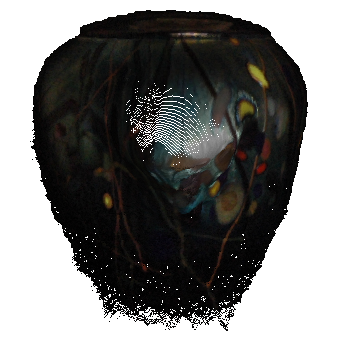
\includegraphics[width=0.2\textwidth]{img/interp/real_interp/vase/vase_ps} \\
Rough surface & Surface hole & Surface spike\\
\end{tabular}
\caption{Visual phenomena that indicate the quality of reconstruction results [better images to be changed].}
\label{fig:vis_quality}
\end{figure*}

% We need to demonstrate that the interpreter would return a reliable reconstructed model given the correct description, and a less successful model given an invalid description. The quality of the reconstruction is determined by comparing the result to the baseline method.

% \subsection{Roadmap}
% [Collect and retrieve data to answer descriptive questions about the activities of the project/programme/policy, the various results it has had, and the context in which it has been implemented.]

% We first need to propose a proof of concept interpreter that is responsible for selecting an appropriate algorithm for reconstruction based on user-specified description. Then we discuss the creation of datasets that are used for evaluation. Finally, we demonstrate the performance of the interpreter by showing the reconstruction results by interpreter-selected algorithm of both synthetic and real-world datasets.

\section{Interpreter}
\label{sec:interp}
Our interface consists of three separate layers. The upper layer is the description of the problem condition. The middle layer is the interpreter which receives a description from the user and return an acceptable result. The bottom layer is the actual implementation of the algorithms. The interpreter is responsible for choosing an appropriate 3D reconstruction algorithm based on the description of the problem domain and additional requirements. Thus, it requires an understanding of algorithmic performance across difference ranges of problem space to create a suitable interpreter.

However, if the interpreter relies solely on the mapping, it is possible that a user-specified description has more than one corresponding algorithm available. We propose to use two additional constraints so that only one appropriate algorithm is selected.

The first constraint is metric-first or shape-first. There are generally two types of reconstruction results: euclidean/metric reconstruction, and shape reconstruction. The former reconstructs a scene with metric information, but generally gives noisier results. The latter can achieve quality that is only matched by laser scanners but lack the depth information. The default setting of this constraint is metric-first.

The second constraint is accuracy-first or completeness-first. Methods that achieve high accuracy do not necessary achieve high completeness. In light of this, the user can choose an algorithm based on the priority level of accuracy and completeness. If multiple algorithm with comparable accuracy or completeness exists, we use a simple ranking system: if one algorithm has the same accuracy but is more complete, or more complete and equally accurate, it is chosen over the others. The default is the accuracy-first constraint.

Thus, the proposed proof of concept interpreter that consists of two components, mapping and constraints, as shown in Figure~\ref{fig:interpreter}. Note that there are many ways of using this mapping information to create an interpreter, and by no means is the proposed one the optimal interpreter. 
\begin{figure}[!htbp]
\centering
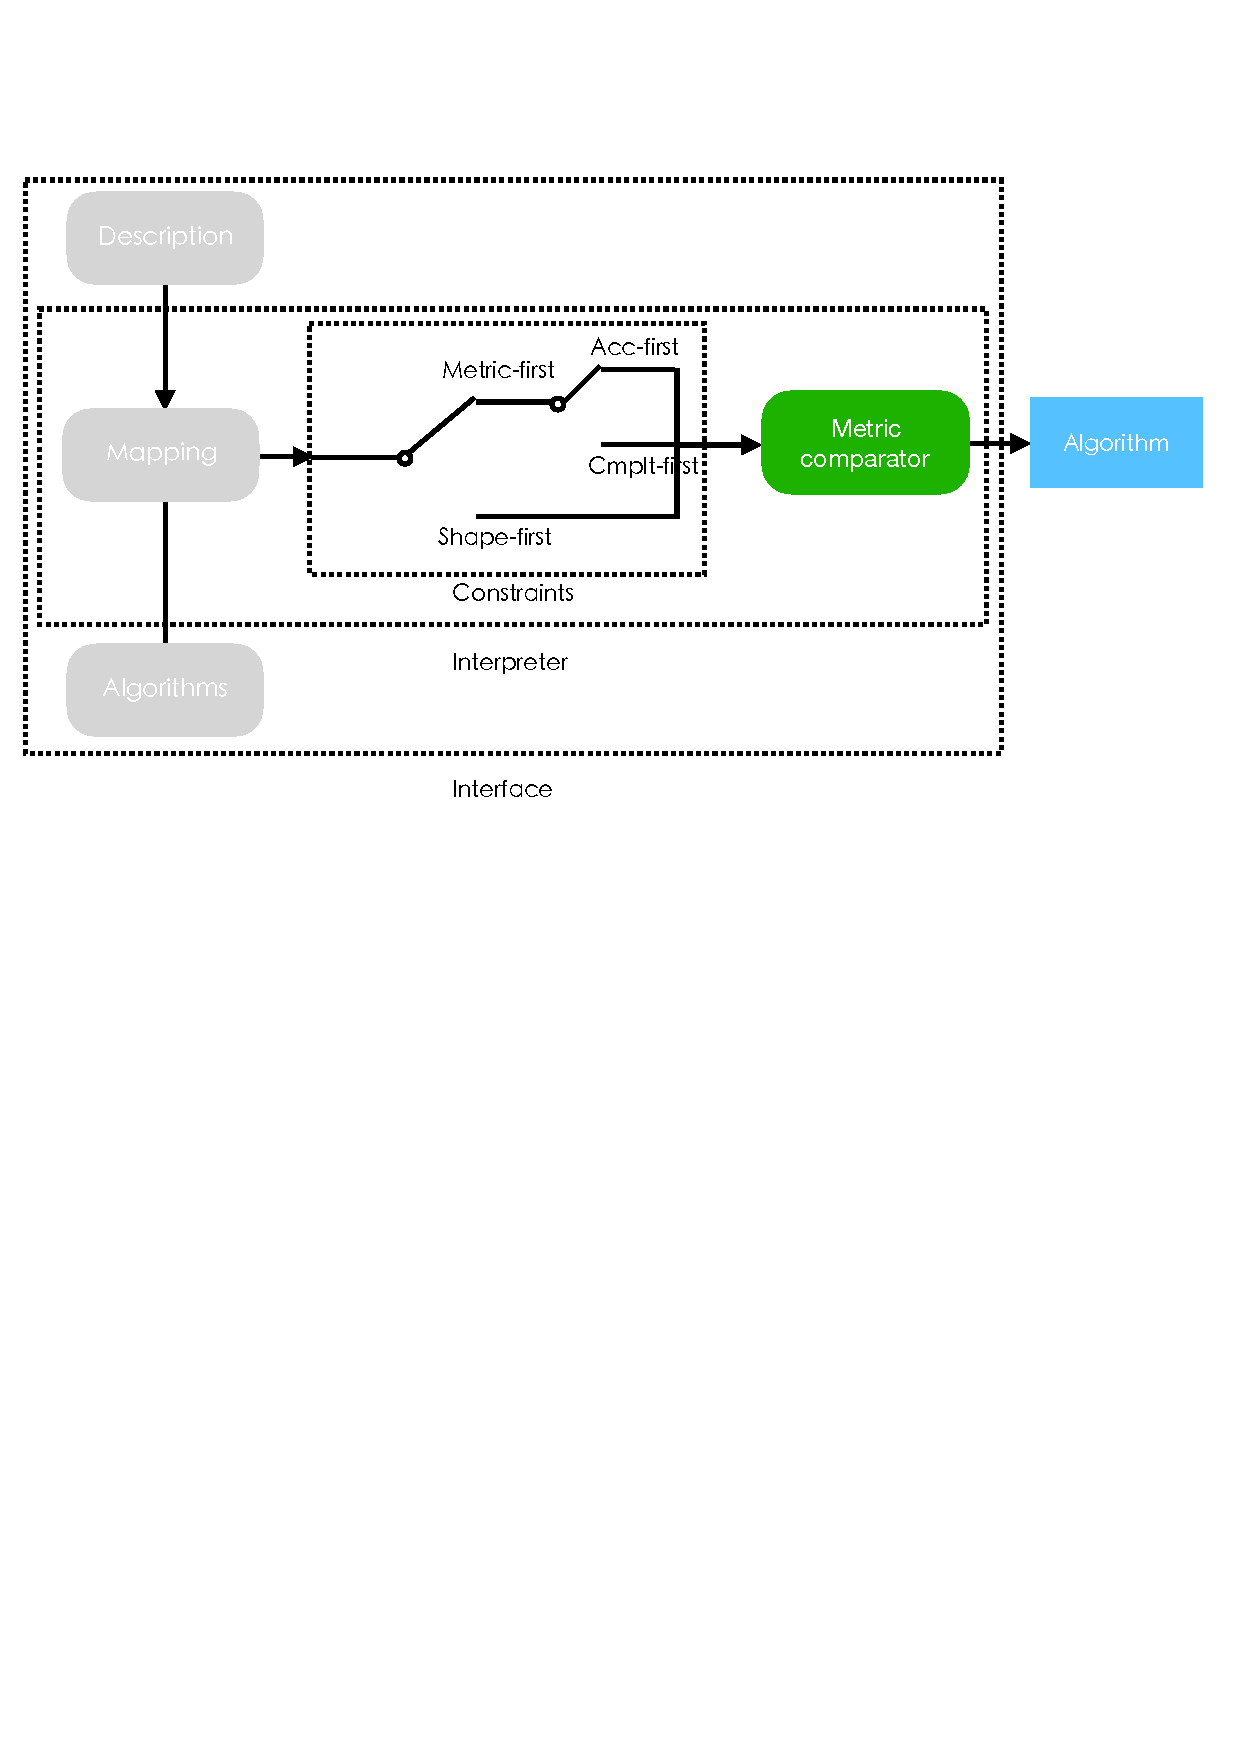
\includegraphics[width=0.8\textwidth]{interp/interpreter.pdf}
\caption{Two components of the Interpreter layer. The metric comparator compares the quantitative measures based on the constraints. If `acc-first' is selected, the comparator favours algorithms with lower accuracy value, whereas if `cmplt-first' is selected, the comparator favours algorithms with higher completeness. If `shape-first' is selected, the comparator favours algorithms with lower angular error.}
\label{fig:interpreter}
\end{figure}

% !!!demonstrate with an example.

% The mapping constructed using the synthetic datasets from Chapter~\ref{ch:3DRecon_Mapping} provides us with a detailed understanding of the performance of algorithms under varied problem conditions. This allows us to select an appropriate algorithm based on a description of properties.

% Next we turn to defining the constraints of the interface. Constraints are provided to allow the user to describe the expected result so that a model best resembling the user's request can be returned by the interface when multiple algorithms achieve satisfactory results. The following constraints are provided: 
% \begin{itemize}
% \item Depth-first/shape-first: methods that reconstructs surface orientations from a single viewpoint cannot retrieve the depth information, and thus are refered to as 2.5D reconstruction. Examples of this are Shape from Shading, Photometric Stereo, and Shape from (de)focus, \etc. However, these methods generally can reconstruct fine scale details, thus can achieve results with much higher quality. Intuitively, depth-first can return model with true depth information whereas shape-first prioritizes fine details over depth information.
% \item Accuracy-first/completeness-first: methods that achieve high accuracy do not necessary achieve high completeness. In light of this, the user can choose an algorithm based on the priority level of accuracy and completeness.
% \end{itemize}

% Under our current interpreter, if a developer-defined description and constraints have more than one corresponding algorithm available, by default, depth-first has higher priority over quality-first, and accuracy has higher priority over completeness. Since GSL typically generates more accurate resutlts, the order of the algorithms is: GSL $>$ PMVS $>$ EPS.

\section{Overview of Datasets}
\label{sec:dataset}
In this section, we introduce a synthetic and a real-world dataset to evaluate the performance of the interpreter under varied problem conditions. To the best of our knowledge, there is few publicly available dataset that capturing images for algorithms across different categories. Most existing datasets target a specific class of algorithms, such as the famous Middlebury dataset~\cite{seitz2006comparison}, DiLiGenT~\cite{shi2016benchmark}, DTU Robot Image Data Sets~\cite{jensen2014large}, and so on. 

The synthetic dataset contains four objects, as shown in Figure~\ref{fig:synth_real_dataset}, and the real-world dataset contains nine objects, four of which are shown in Figure~\ref{fig:synth_real_dataset}. Please refer to Figure~\ref{fig:real_data_material} for the complete dataset. It covers materials that are representative of four problem conditions proposed in Chapter~\ref{ch:3DRecon_ProbSpace}: textureless-diffuse-bright (bust, statue), textureless-mixed-bright (vase0, cup), textured-diffuse-bright (barrel, pot), textured-mixed-bright (vase1, vase). In terms of surface shapes, we have focused mainly on objects with simple geometric properties, namely, smoothly curved surfaces with shallow concavities, see descriptions and example images in Figure~\ref{fig:synth_real_dataset}.
\begin{figure*}[!htbp]
\centering
\begin{tabular}{l*{4}{c}}
\toprule
\parbox[t]{2mm}{\multirow{3}{*}{\rotatebox[origin=c]{90}{Appearance}}}
& \tabitem textureless & \tabitem textureless & \tabitem textured & \tabitem textured\\
& \tabitem diffuse & \tabitem mixed d/s & \tabitem diffuse & \tabitem mixed d/s\\
& \tabitem bright & \tabitem bright & \tabitem bright & \tabitem bright\\\\ \cline{2-5}
& 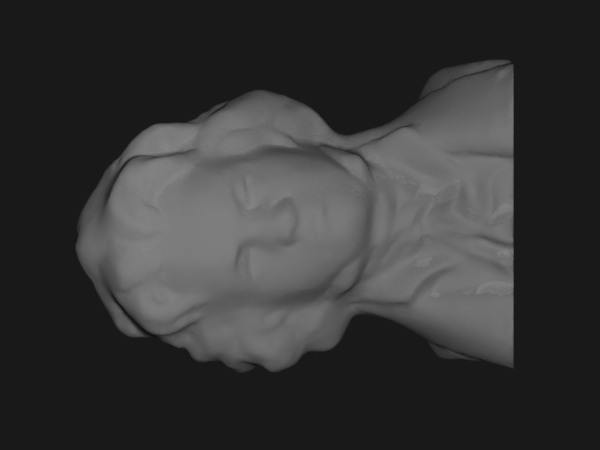
\includegraphics[width=0.2\textwidth]{interp/synth_data/bust} &
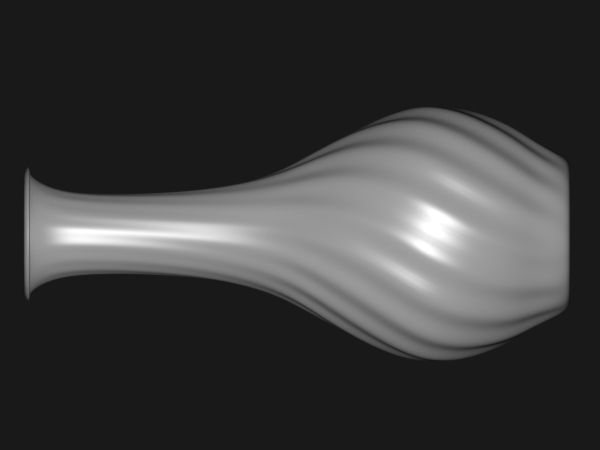
\includegraphics[width=0.2\textwidth]{interp/synth_data/vase0} &
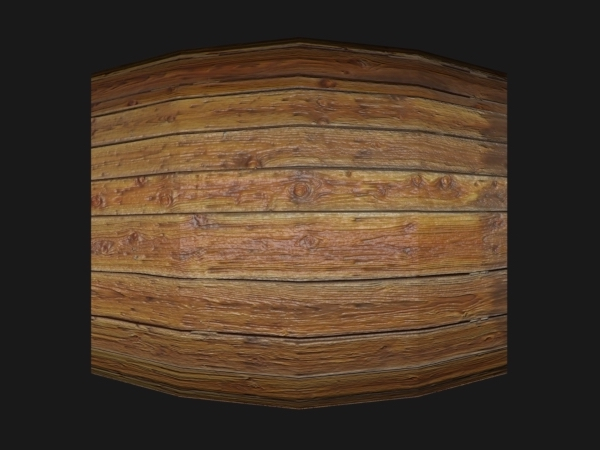
\includegraphics[width=0.2\textwidth]{interp/synth_data/barrel} &
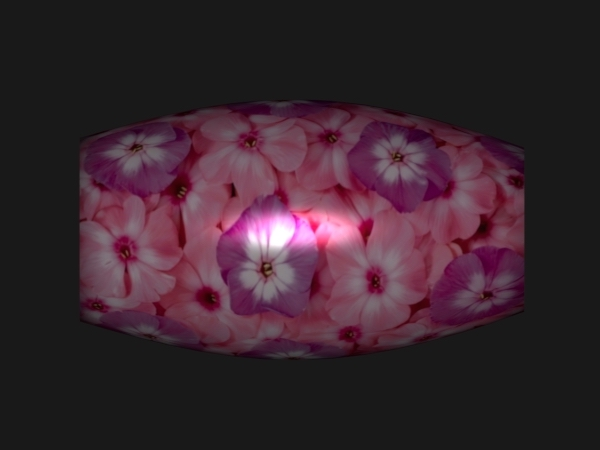
\includegraphics[width=0.2\textwidth]{interp/synth_data/vase1}\\
& (a). bust & (b). vase0 & (c). barrel & (d). vase1\\
& 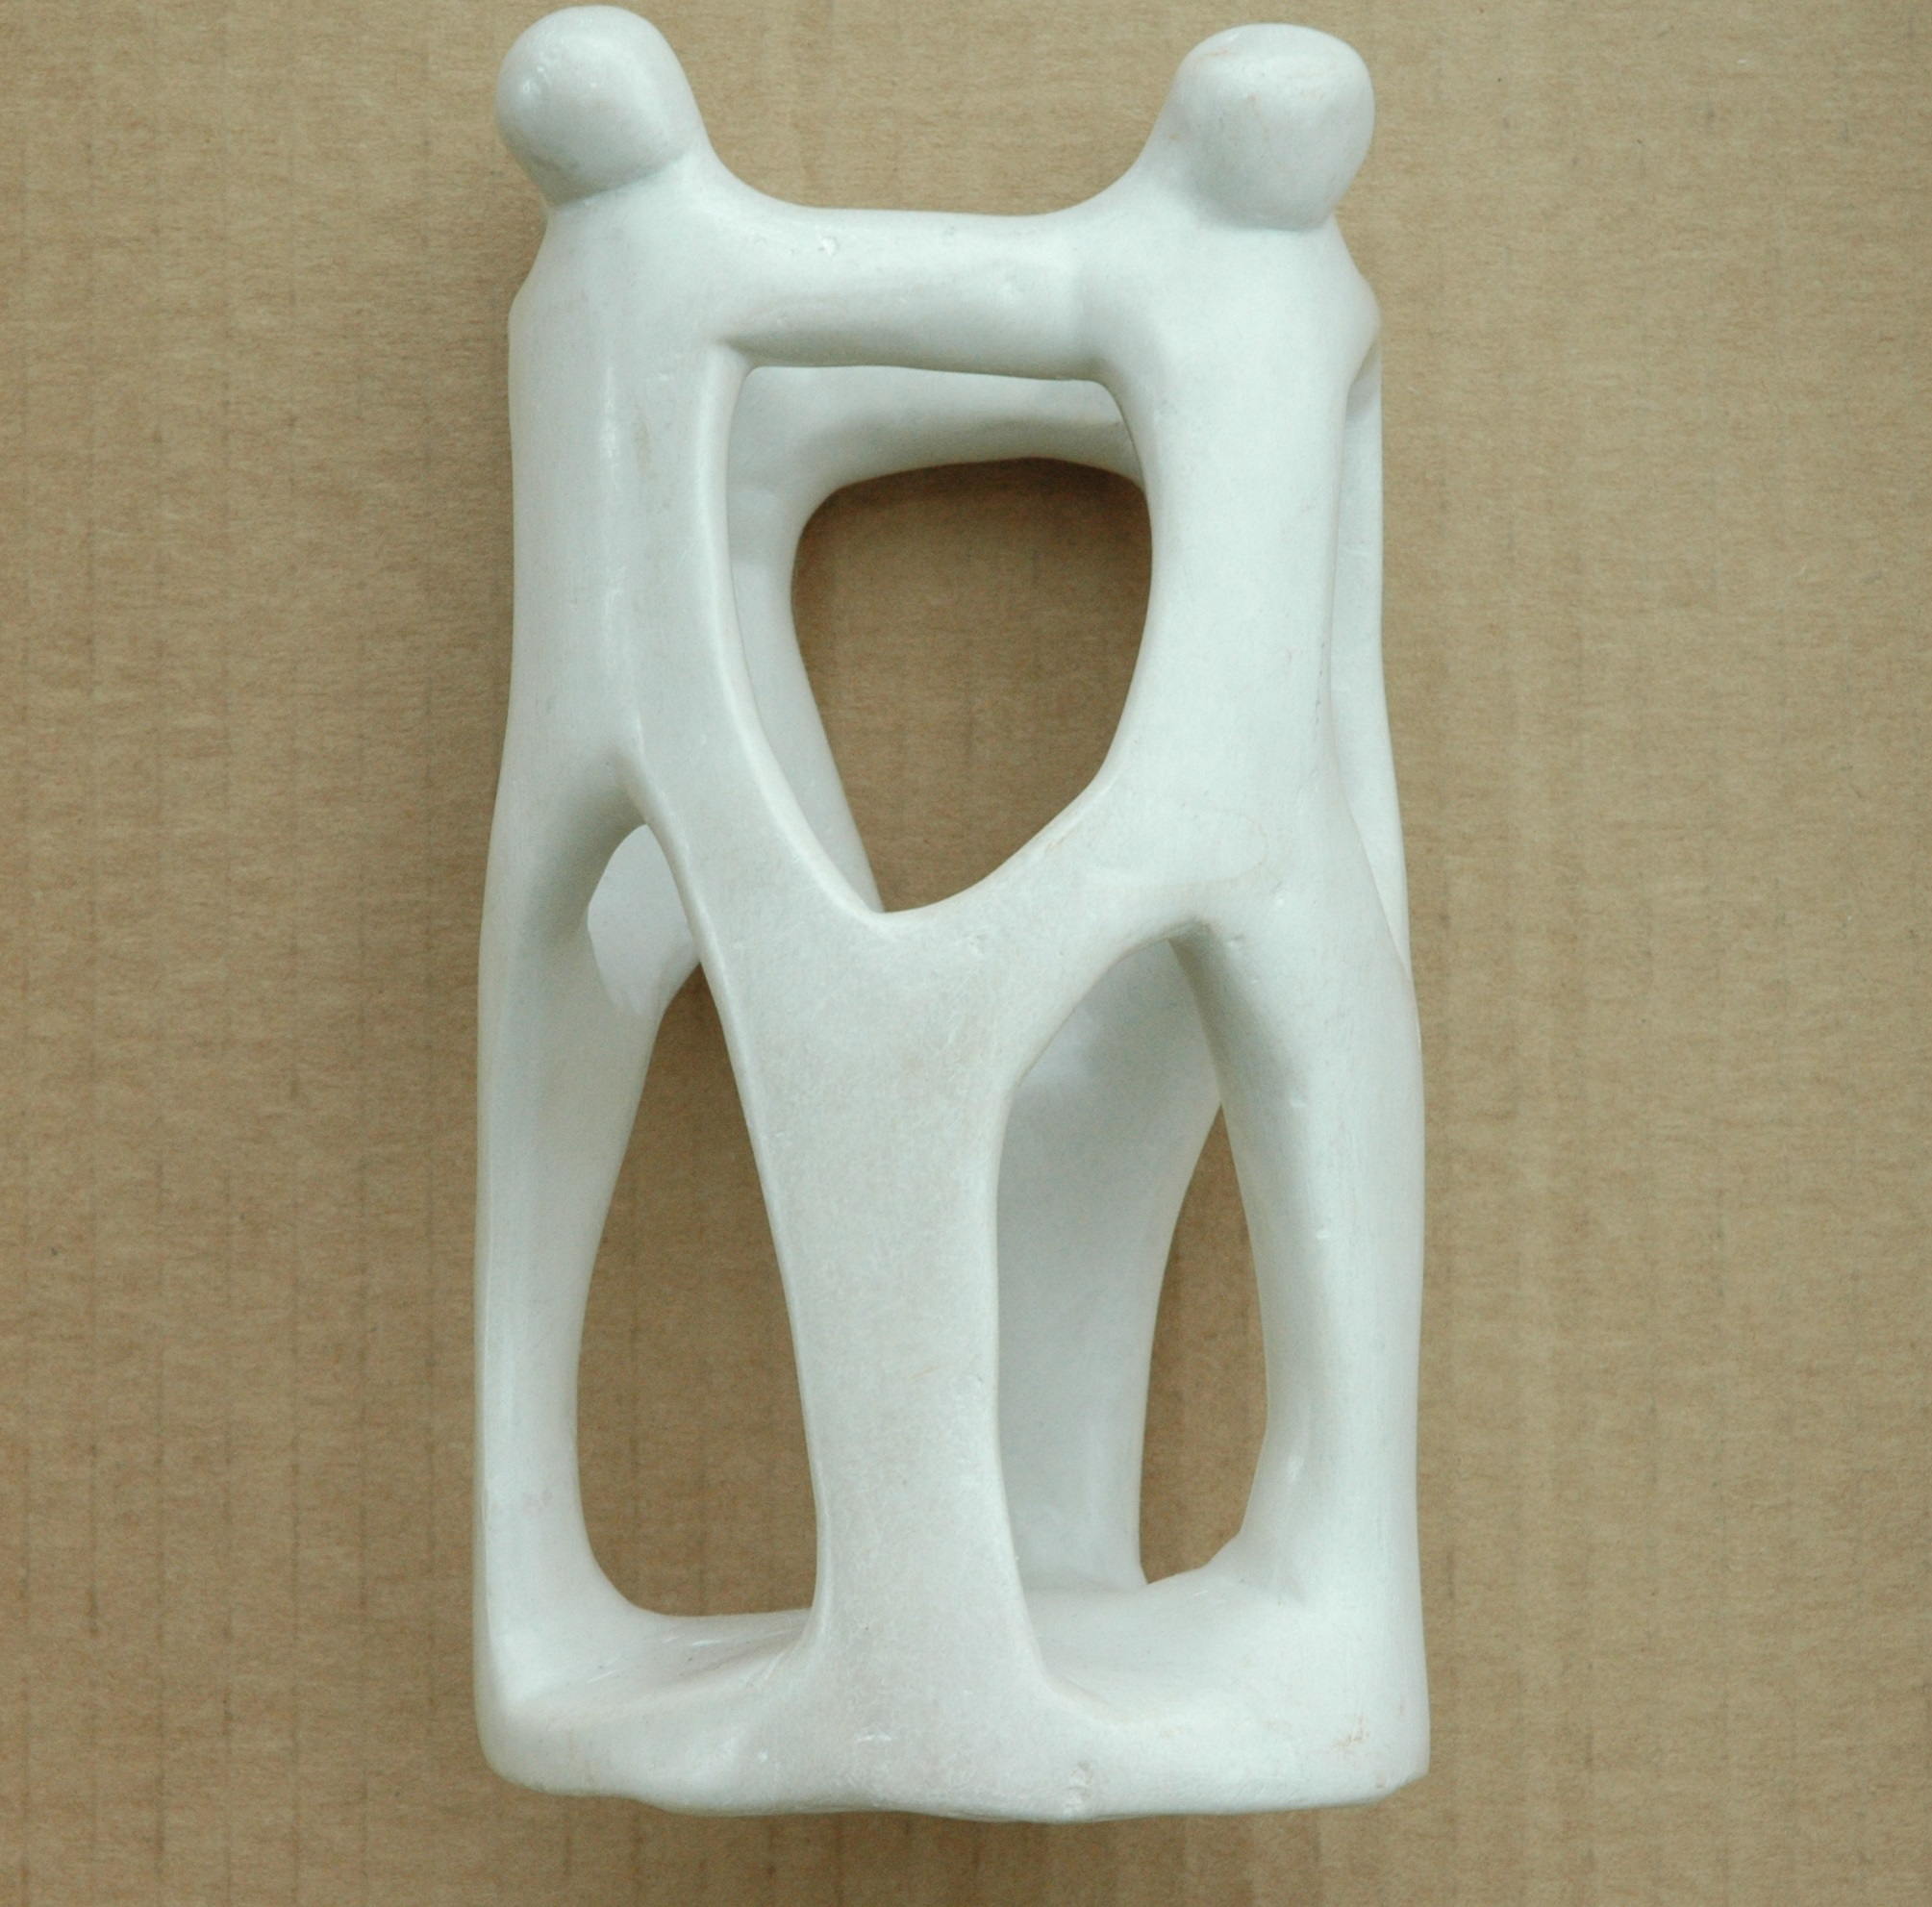
\includegraphics[width=0.2\textwidth]{interp/real_world_img/statue/statue} &
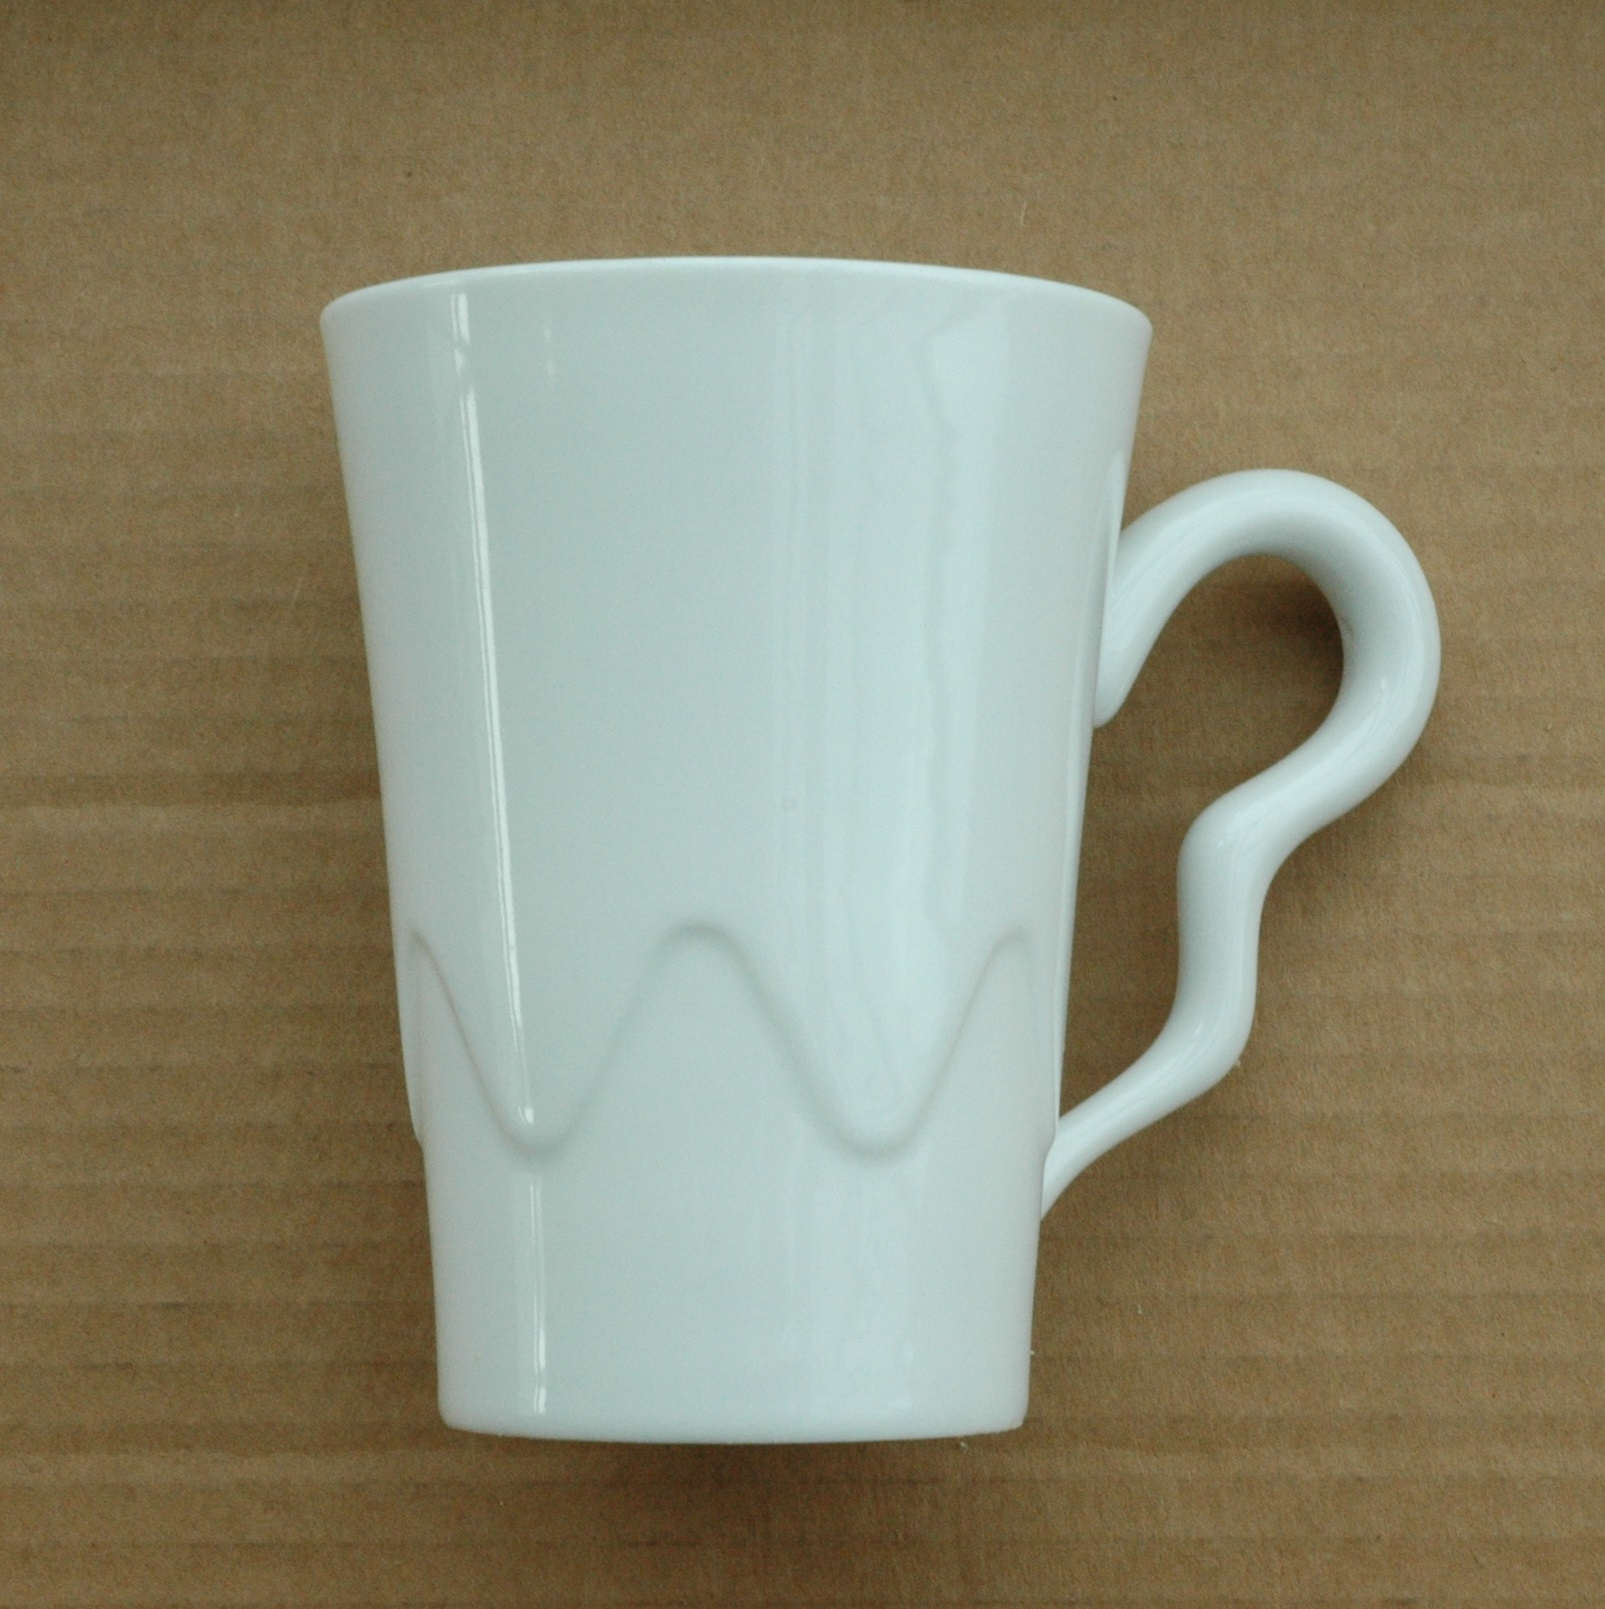
\includegraphics[width=0.2\textwidth]{interp/real_world_img/cup/cup} &
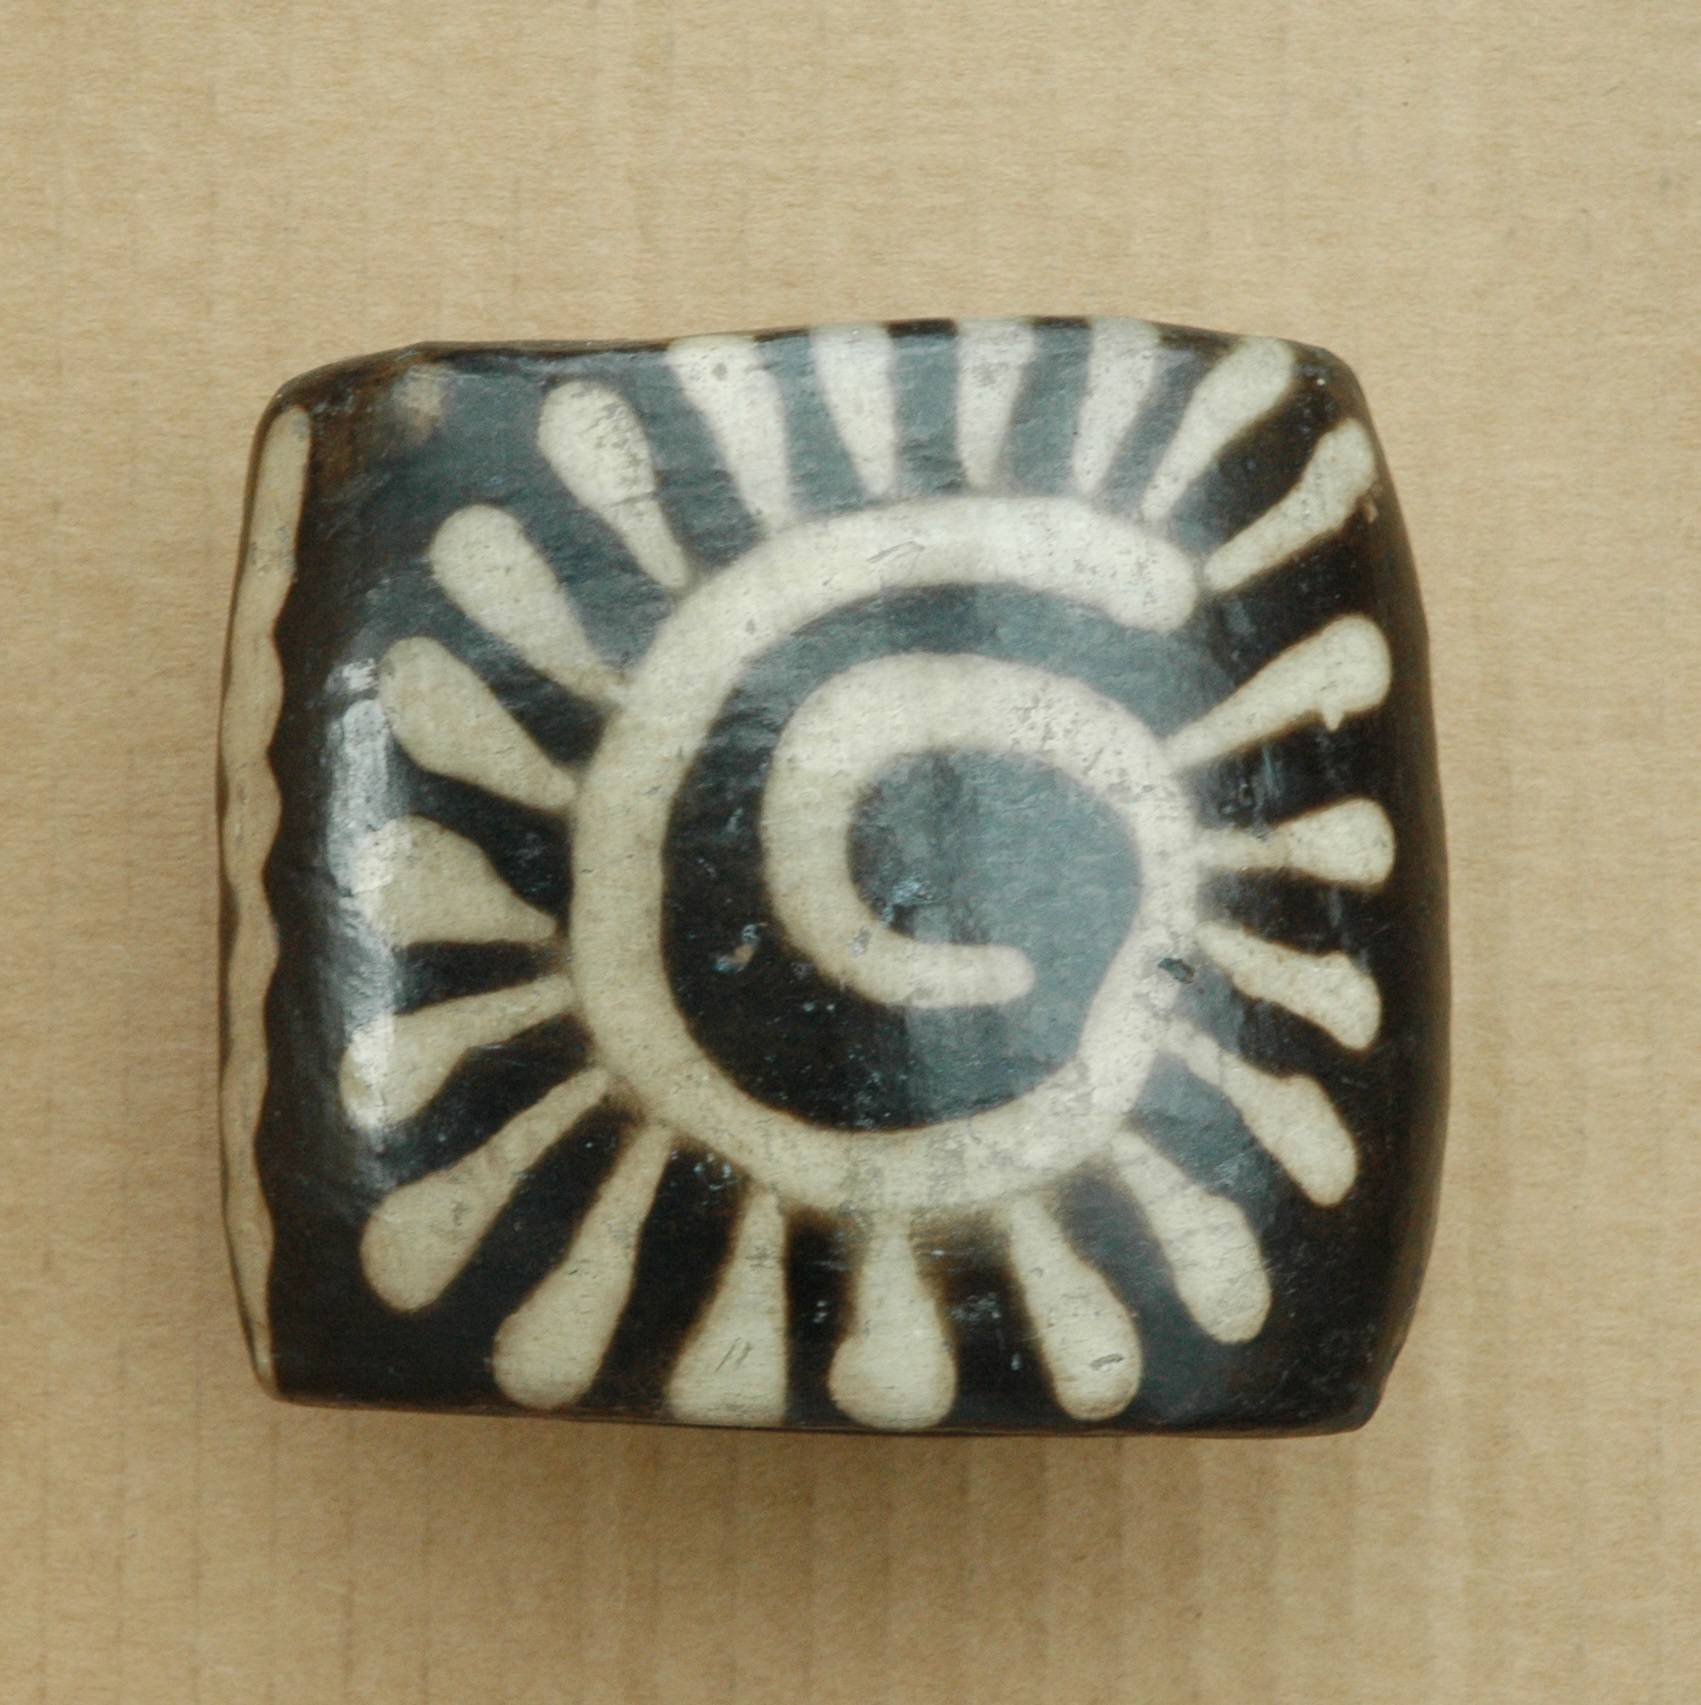
\includegraphics[width=0.2\textwidth]{interp/real_world_img/pot/pot} &
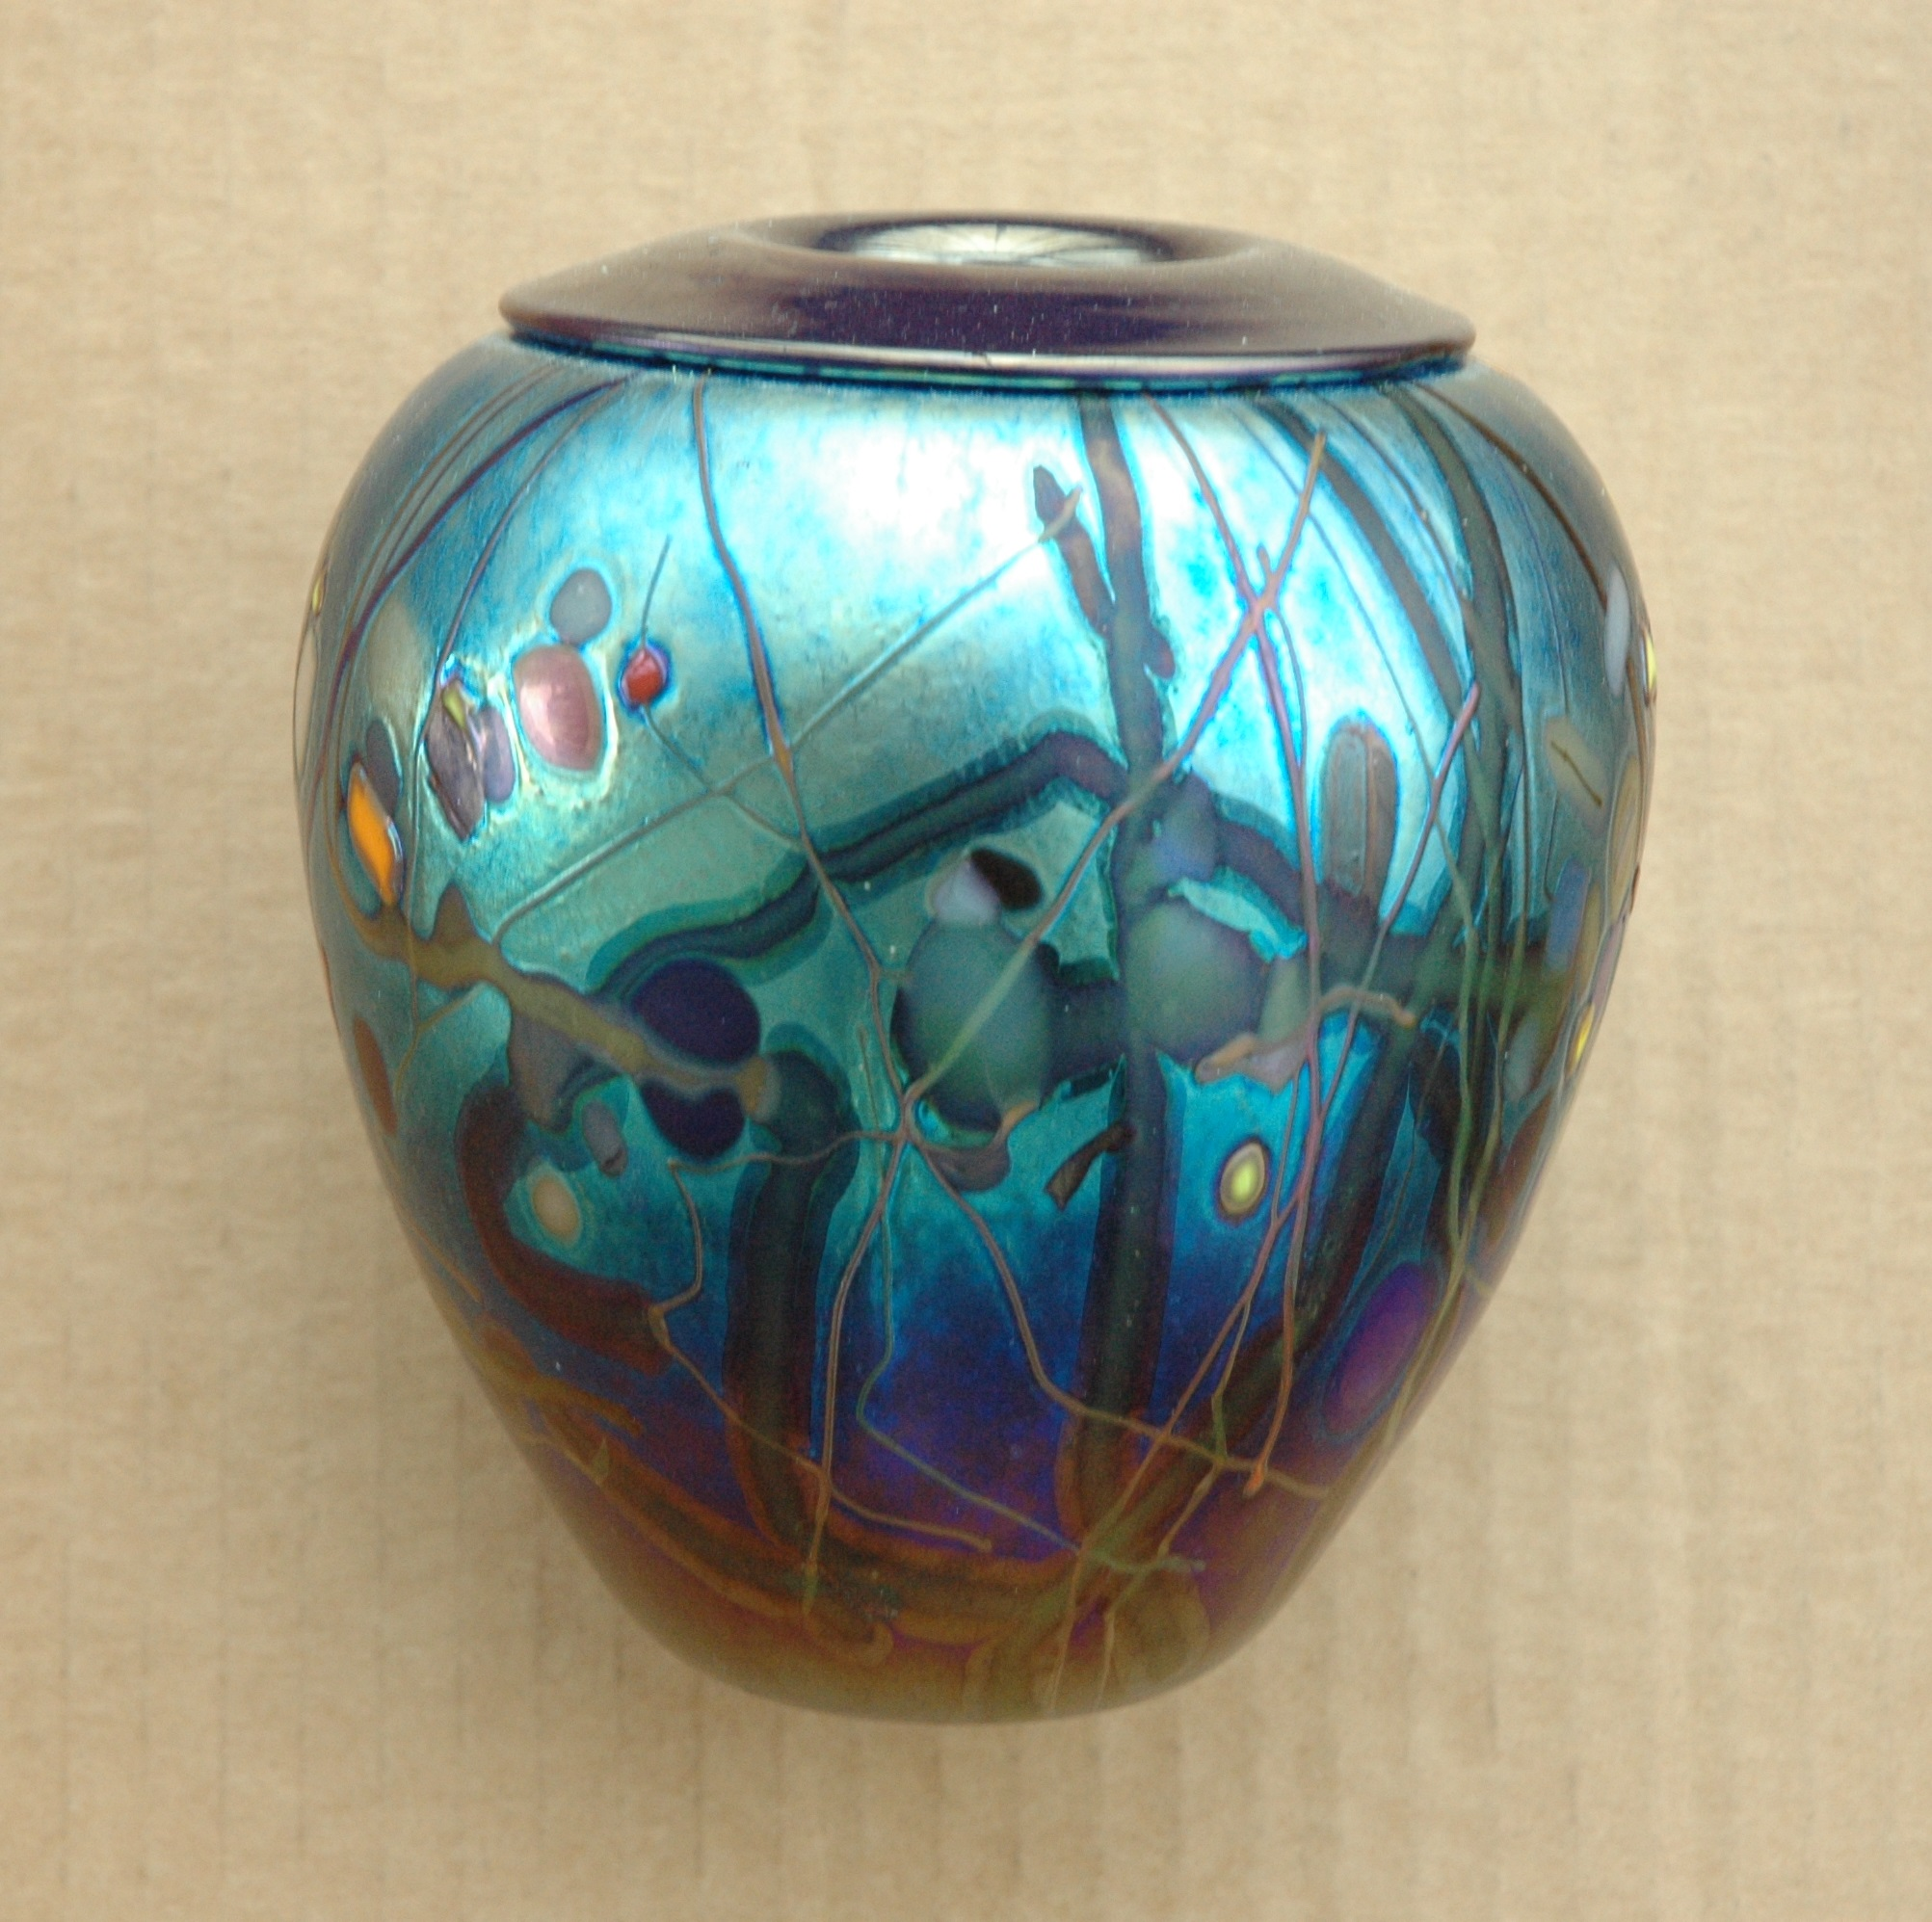
\includegraphics[width=0.2\textwidth]{interp/real_world_img/vase/vase} \\
& (e). statue & (f). cup & (g). pot & (h). vase\\
\end{tabular}
\caption{Representative objects of the four problem condition discussed in Chapter~\ref{ch:3DRecon_ProbSpace}. (a)-(d): Synthetic objects, and (e)-(h) real-world objects.}
\label{fig:synth_real_dataset}
\end{figure*}

\subsection{Calibration}
For MVS, a calibration pattern proposed in~\cite{li2013multiple} is imaged under the object, which is used for calibrating the camera position and orientation by Structure from Motion softwares, such as VisualSfM~\cite{wu2011visualsfm}. The focal length is known a priori and remains fixed duing the image capturing process. Thus the extrinsic parameters of the camera can be retrieved up to a similarity transformation, and the reconstruction result is a metric/euclidean recontruction.

For most PS algorithms, \ie calibrated PS algorithms, it is necessary to estimate the light direction and intensity. However, the selected PS algorithm can deal with unknown light sources and spatially-varying BRDFs. Thus, light calibration is not a required step. Though it is preferable to correct the non-linear response of camera, \citeauthor{hertzmann2005example} discovered that it was unnecessary for EPS. Thus, we did not perform the radiometric calibration step. No geometric calibration of the camera is needed.

For SL, a opensource camera-projector calibration software developed by~\citeauthor{moreno2012simple} is used for calibration. This technique works by projecting temporal patterns onto the calibration pattern, and uses local homography to individually translate each checkerboard corner from the camera plane to the projector plane. This technique can estimate both the intrinsic parameter and camera and projector, and the relative position and orientation.

\subsection{Image capturing}
The creation of synthetic dataset is largely the same as that discussed in Chapter~\ref{ch:3DRecon_Mapping}, thus is omitted in this section. The images of real-world dataset are captured using a Nikon D70S camera with a $18-70mm$ lens. The image resolution is $3004\times 2000$ pix.

For MVS, we capture the dataset by positioning the camera in three different heights. The objects are about $30-50cm$ away from the camera, and stays fixed on a turntable. We have followed the following two steps to acquire data: 1) put the camera at a different height, adjust the orientation so that the object in at the center of the frame; 2) take pictures while rotating the table. The table rotates approximately $30^\circ$ every time. We rotate it 12 times and in total, we can obtain 12 image per height.

For PS, a $70-200mm$ lens, a handheld lamp, and two reference objects (diffuse and glossy) are used. The objects are positioned about $3m$ from the camera to approximate orthographic projection. To avoid inter-reflection, all data are captured in a dark room with everying covered by black cloth except the target object. We use a hand-held lamp as the light source and choose close to frontal viewpoints to avoid severe self-shadowing effect. We take 20 images per object and select 15 plus images depending on the severity of the self-shadow effect.

For SL, we use a Sanyo Pro xtraX Multiverse projector with a resolution of $1024\times 768$. The baseline angle of the camera projector pair is approximately $10^\circ$. To alleviate the effect of ambient light, all images are captured with room lights off. To counteract the effect of inter-reflection, additional images are captured by projecting an all-white and all-black patterns.

\subsection{Synthetic dataset}
Each object in the synthetic dataset represents one of the four problem conditions discussed in Section~\ref{ch:3DRecon_ProbSpace}. The description of problem condition of each synthetic object is shown in Figure~\ref{fig:synth_data}, as well as the appropriate algorithm selected by the interpreter. Given a user specified description, the proof of concept interpreter will select an algorithm, and any object that matches this description should be well reconstructed by this selected algorithm.
% Since a description could be mapped to multiple algorithms, an object that does not match the description could potentially have a successful reconstruction result as well.
\begin{figure}[!htbp]
\centering
\begin{tabular}{cl|*{4}{p{2.2cm}}}
\toprule
\multicolumn{2}{c}{Class \#} & 1 & 2 & 3 & 4\\
\midrule
\parbox[t]{2mm}{\rotatebox[origin=c]{90}{Objects}} & &
\raisebox{-.5\height}{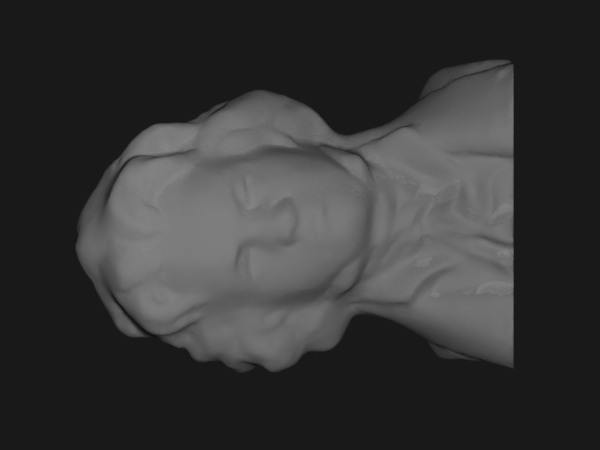
\includegraphics[width=0.15\textwidth]{interp/synth_data/bust}} &
\raisebox{-.5\height}{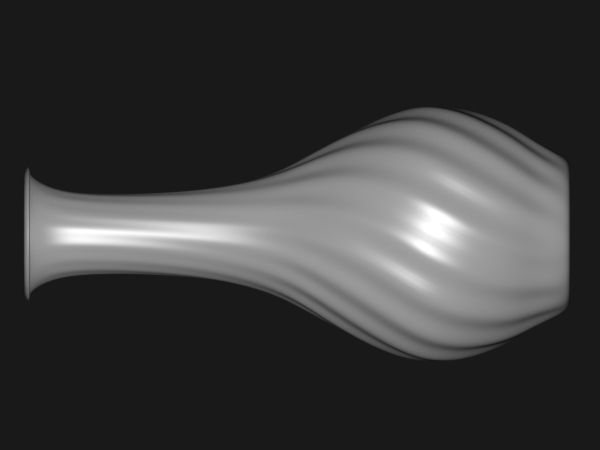
\includegraphics[width=0.15\textwidth]{interp/synth_data/vase0}} &
\raisebox{-.5\height}{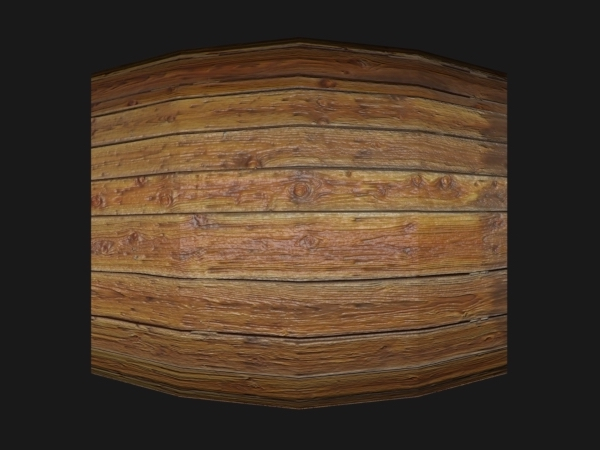
\includegraphics[width=0.15\textwidth]{interp/synth_data/barrel}} &
\raisebox{-.5\height}{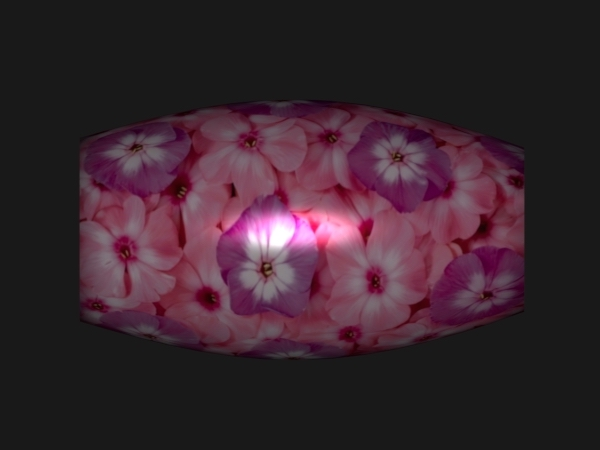
\includegraphics[width=0.15\textwidth]{interp/synth_data/vase1}}\\ \cline{3-6}
\parbox[t]{2mm}{\multirow{3}{*}{\rotatebox[origin=c]{90}{Semantic}}}
& & \tabitem textureless & \tabitem textureless & \tabitem textured & \tabitem textured\\
& & \tabitem diffuse & \tabitem mixed d/s & \tabitem diffuse & \tabitem mixed d/s\\
& & \tabitem bright & \tabitem bright & \tabitem bright & \tabitem bright\\ \cline{3-6}
\parbox[t]{2mm}{\multirow{4}{*}{\rotatebox[origin=c]{90}{Description}}}
& Tex & 0.2 & 0.2 & 0.8 & 0.8\\
& Alb & 0.8 & 0.8 & 0.8  & 0.8\\
& Spec & 0.2 & 0.8 & 0.2 & 0.8\\
& Rough & 0.8 & 0.2 & 0.2 & 0.2\\ \cline{3-6}
\parbox[t]{2mm}{\multirow{2}{*}{\rotatebox[origin=c]{90}{Alg}}}
& & \tabitem EPS & \tabitem\tc{EPS} & \tabitem PMVS & \tabitem\tc{PMVS} \\
& & \tabitem\tc{GSL} &  & \tabitem EPS & \tabitem EPS\\
& & & & \tabitem\tc{GSL} & \\
\bottomrule
\end{tabular}
\caption{The repsentatives of the four classes of objects used for evaluation. Example images and problem conditions of synthetic objects are in the first two rows. The correct description that matches the problem condition of corresponding object is presented in third row. The last row shows the algorithms returned by the mapping, from which the interpreter selects one successful algorithm, which is in colour red.}
\label{fig:synth_data}
\end{figure}

\subsection{Real-world Dataset}
We select four real-world objects, each represents the one of the four problem condtiions proposed in Chapter~\ref{ch:3DRecon_ProbSpace}, as shown in Figure~\ref{fig:real_data}. The descriptions of problem conditions of real-world objects are shown in Figure~\ref{fig:real_data}, as well as the appropriate algorithm selected by the interpreter. Given a user specified description, the proof of concept interpreter will select an algorithm, and any object that matches this description should be well reconstructed by this selected algorithm.
\begin{figure}[!htbp]
\centering
\begin{tabular}{cl|*{4}{p{2.2cm}}}
\toprule
\multicolumn{2}{c}{Class \#} & 1 & 2 & 3 & 4\\
\midrule
\parbox[t]{2mm}{\rotatebox[origin=c]{90}{Objects}} & &
\raisebox{-.5\height}{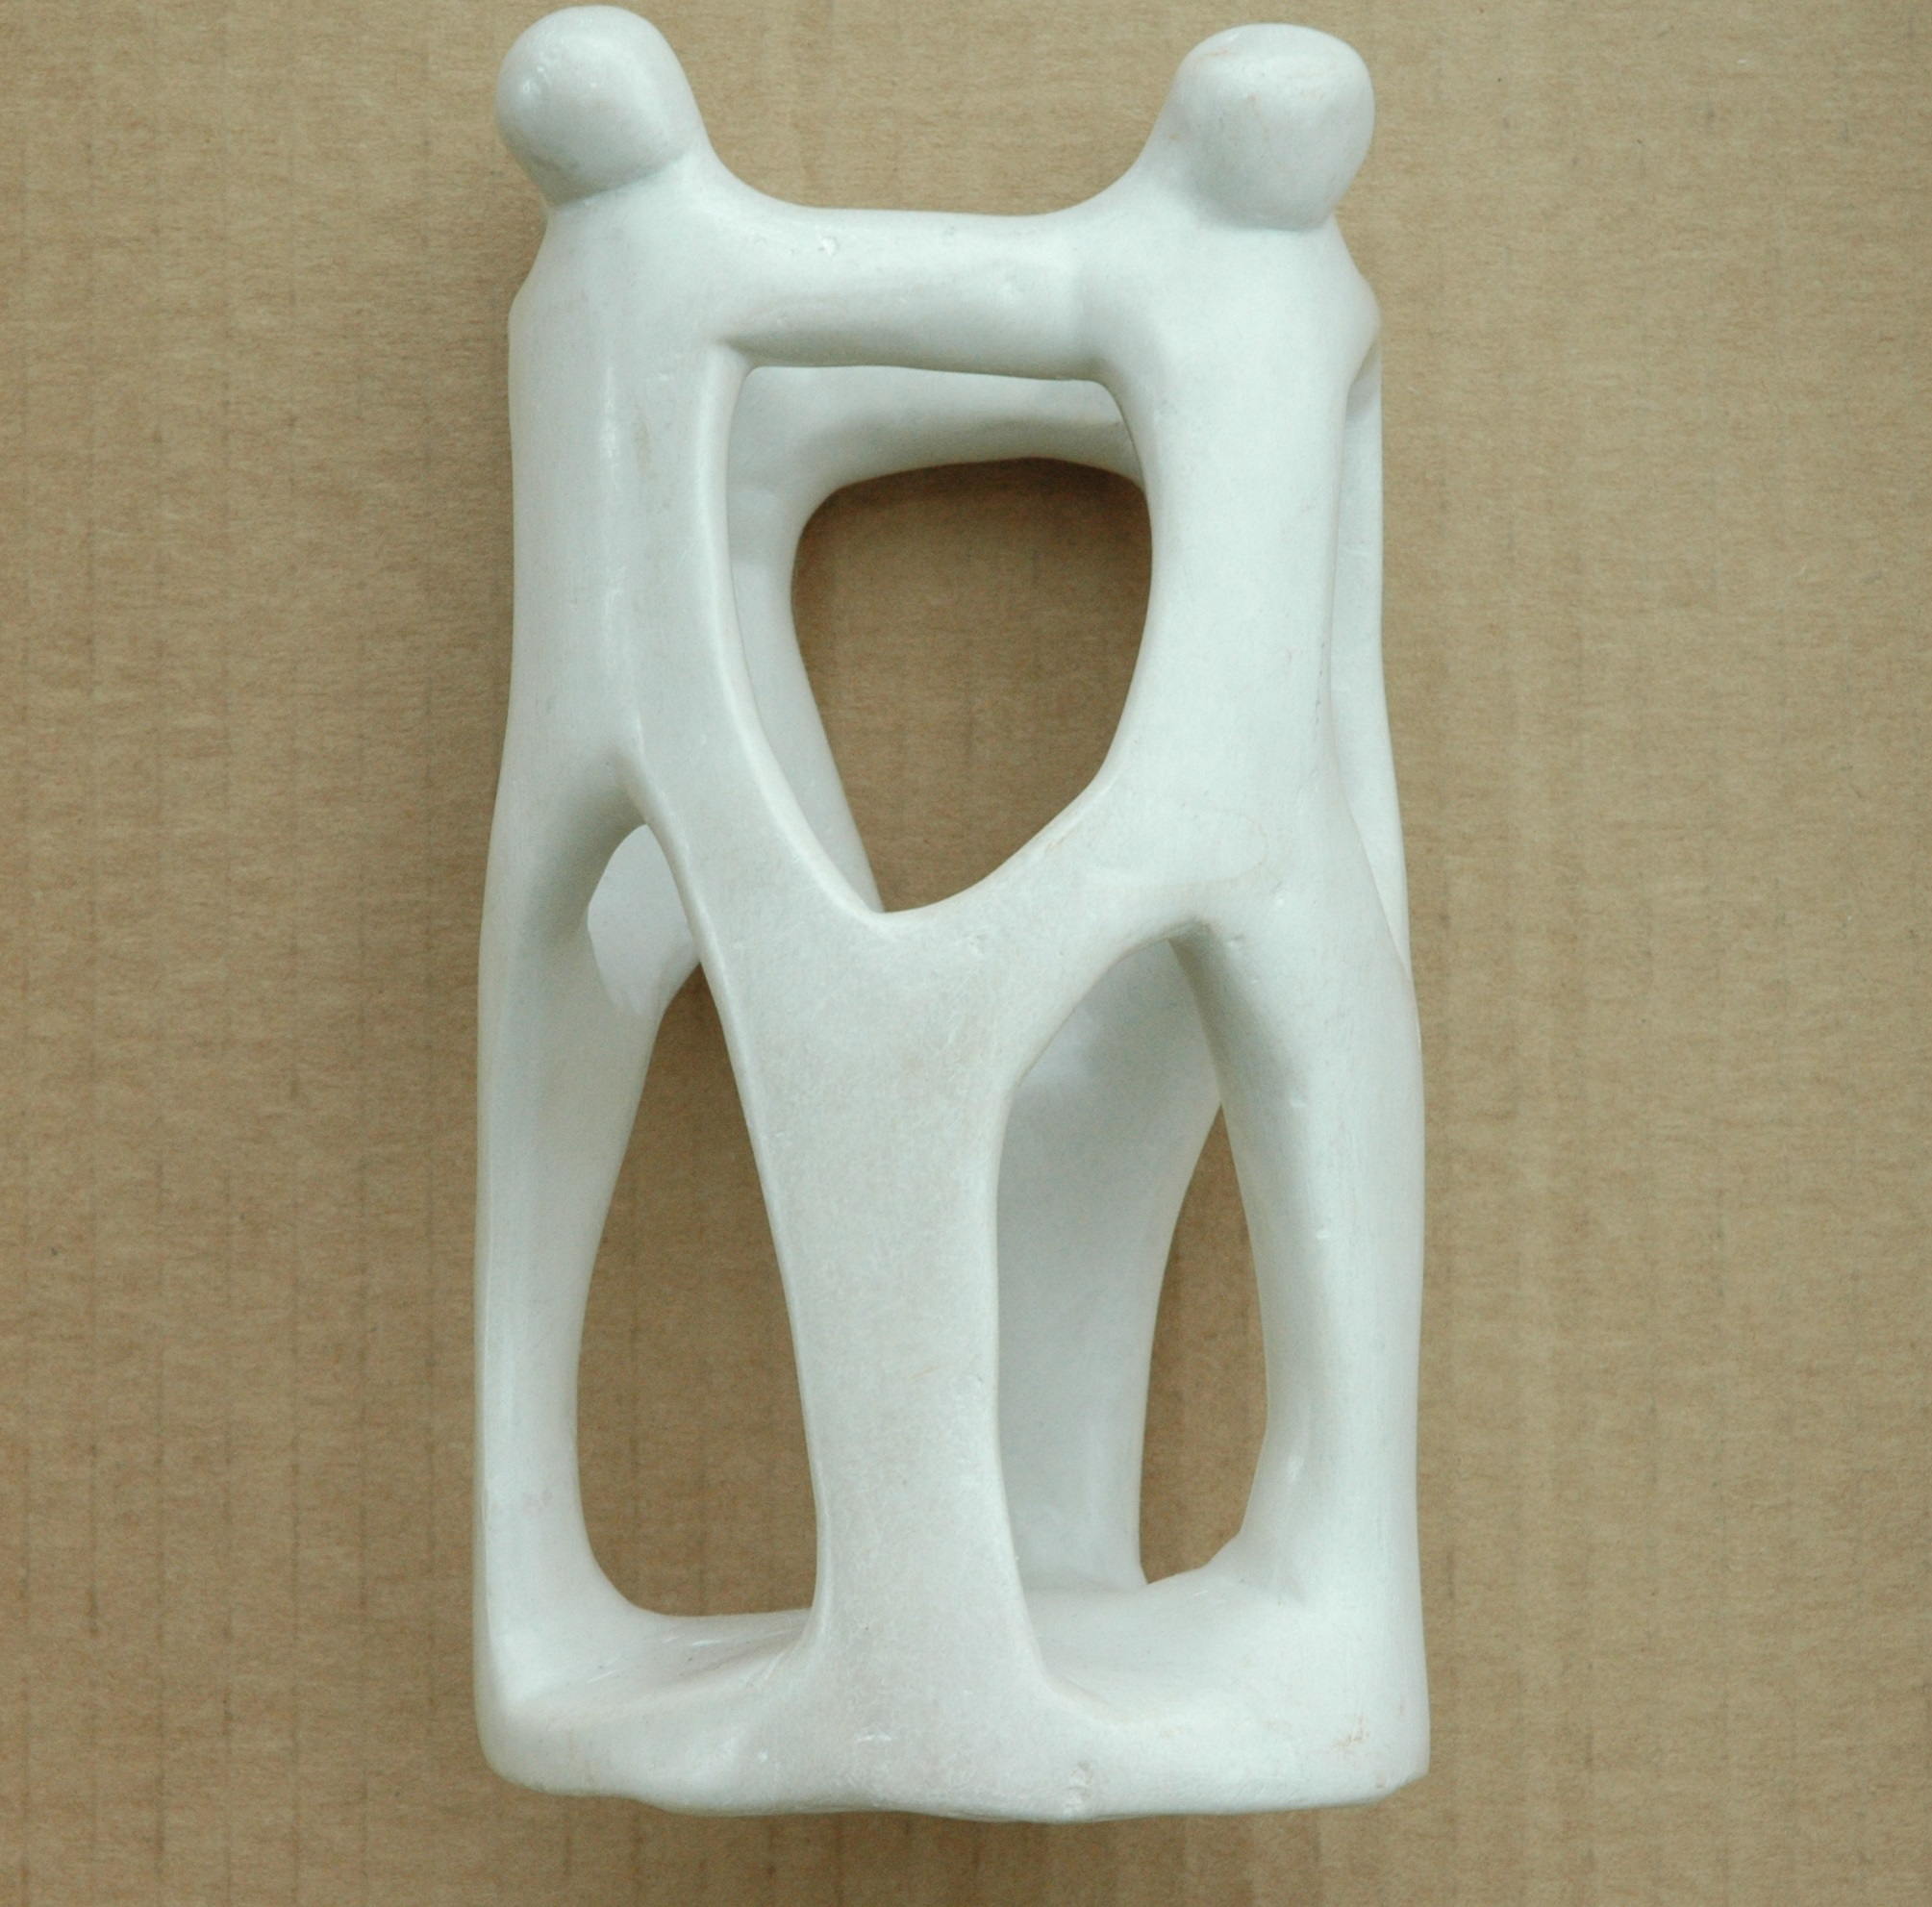
\includegraphics[width=0.15\textwidth]{interp/real_world_img/statue/statue}} &
\raisebox{-.5\height}{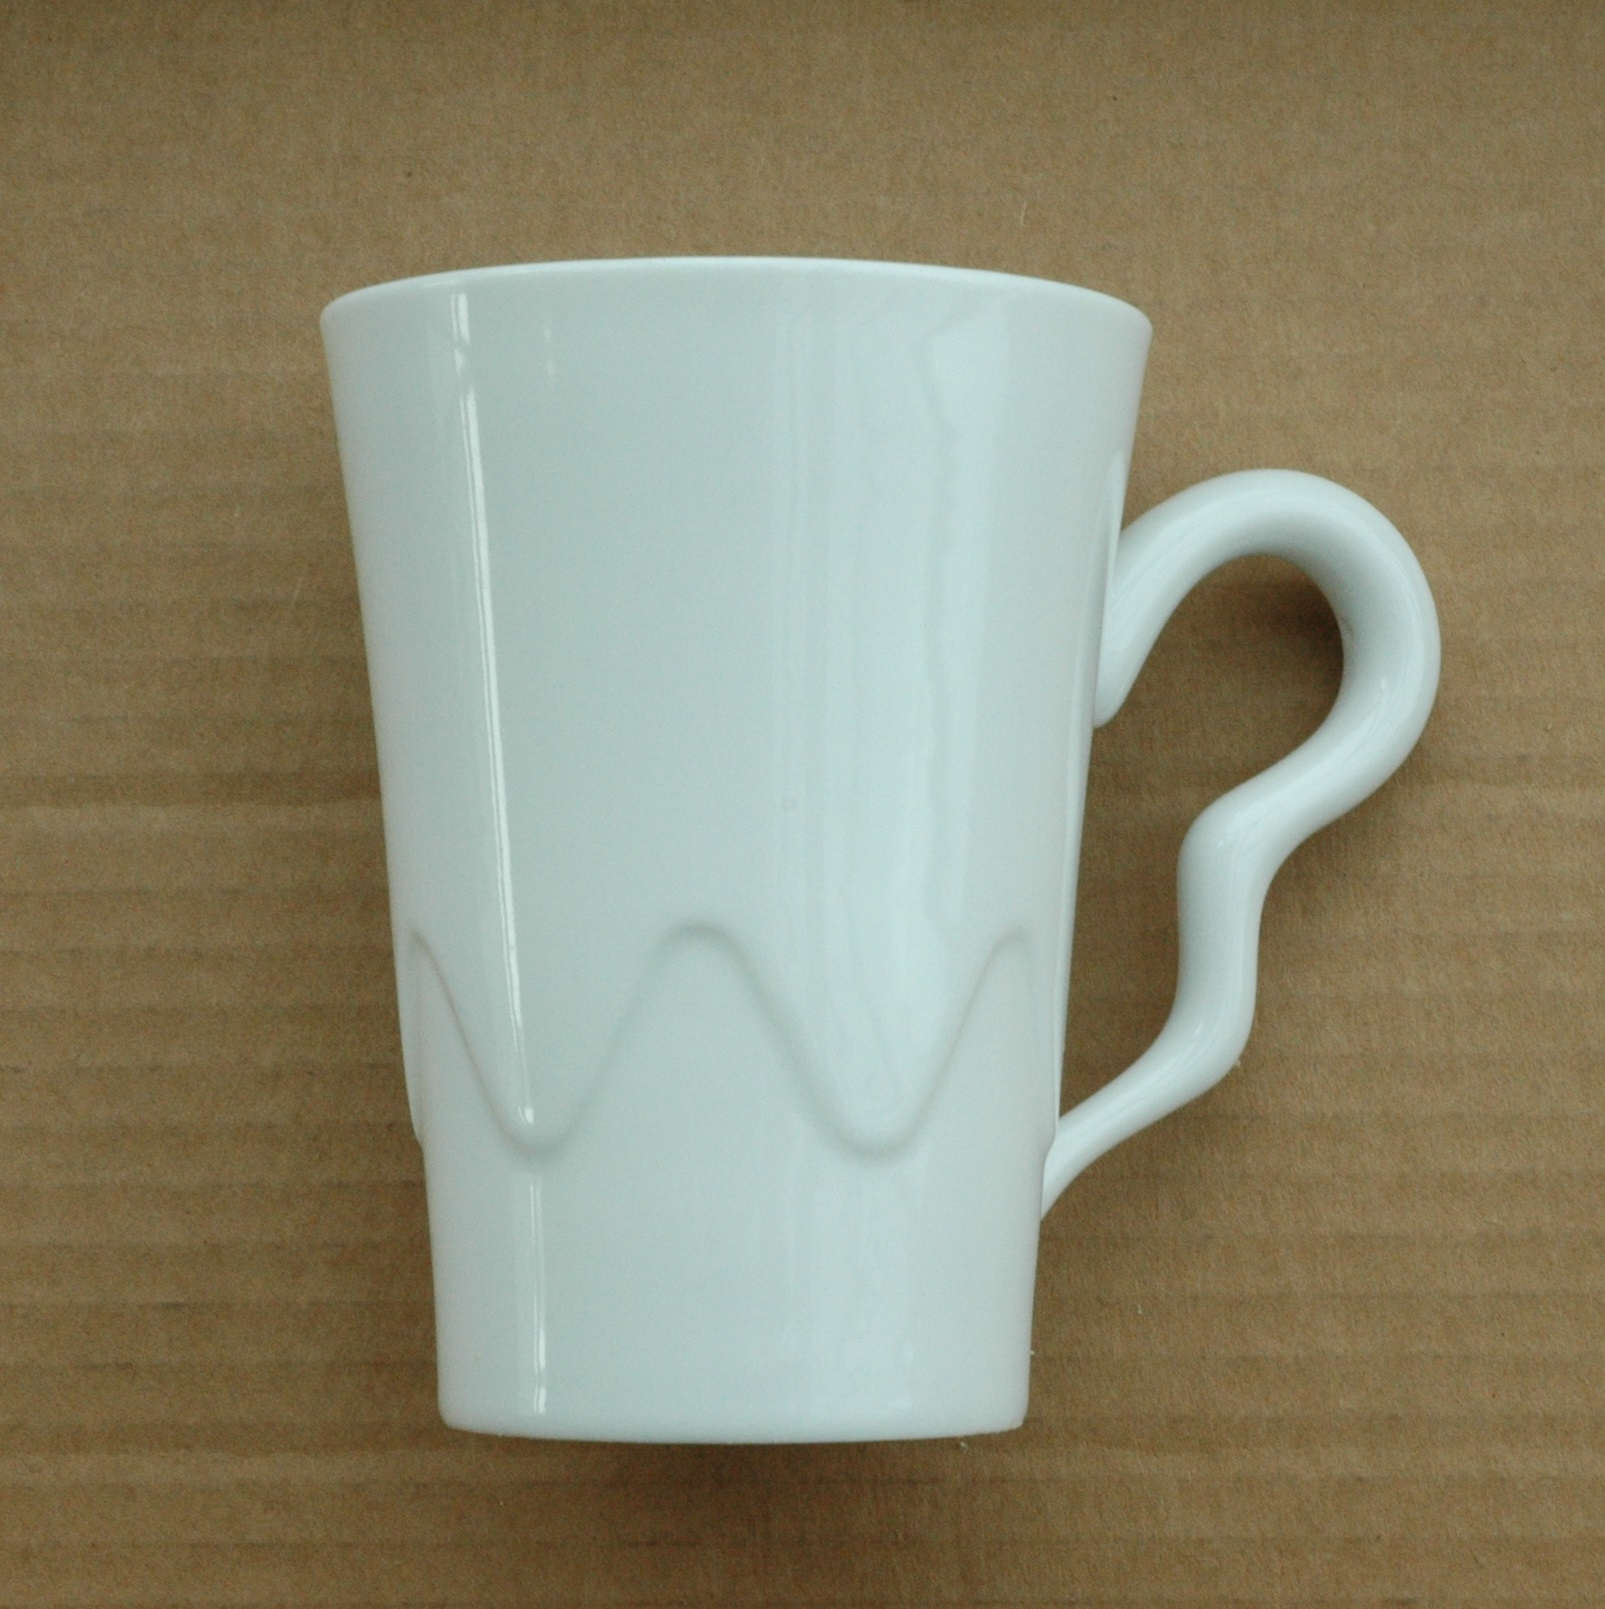
\includegraphics[width=0.15\textwidth]{interp/real_world_img/cup/cup}} &
\raisebox{-.5\height}{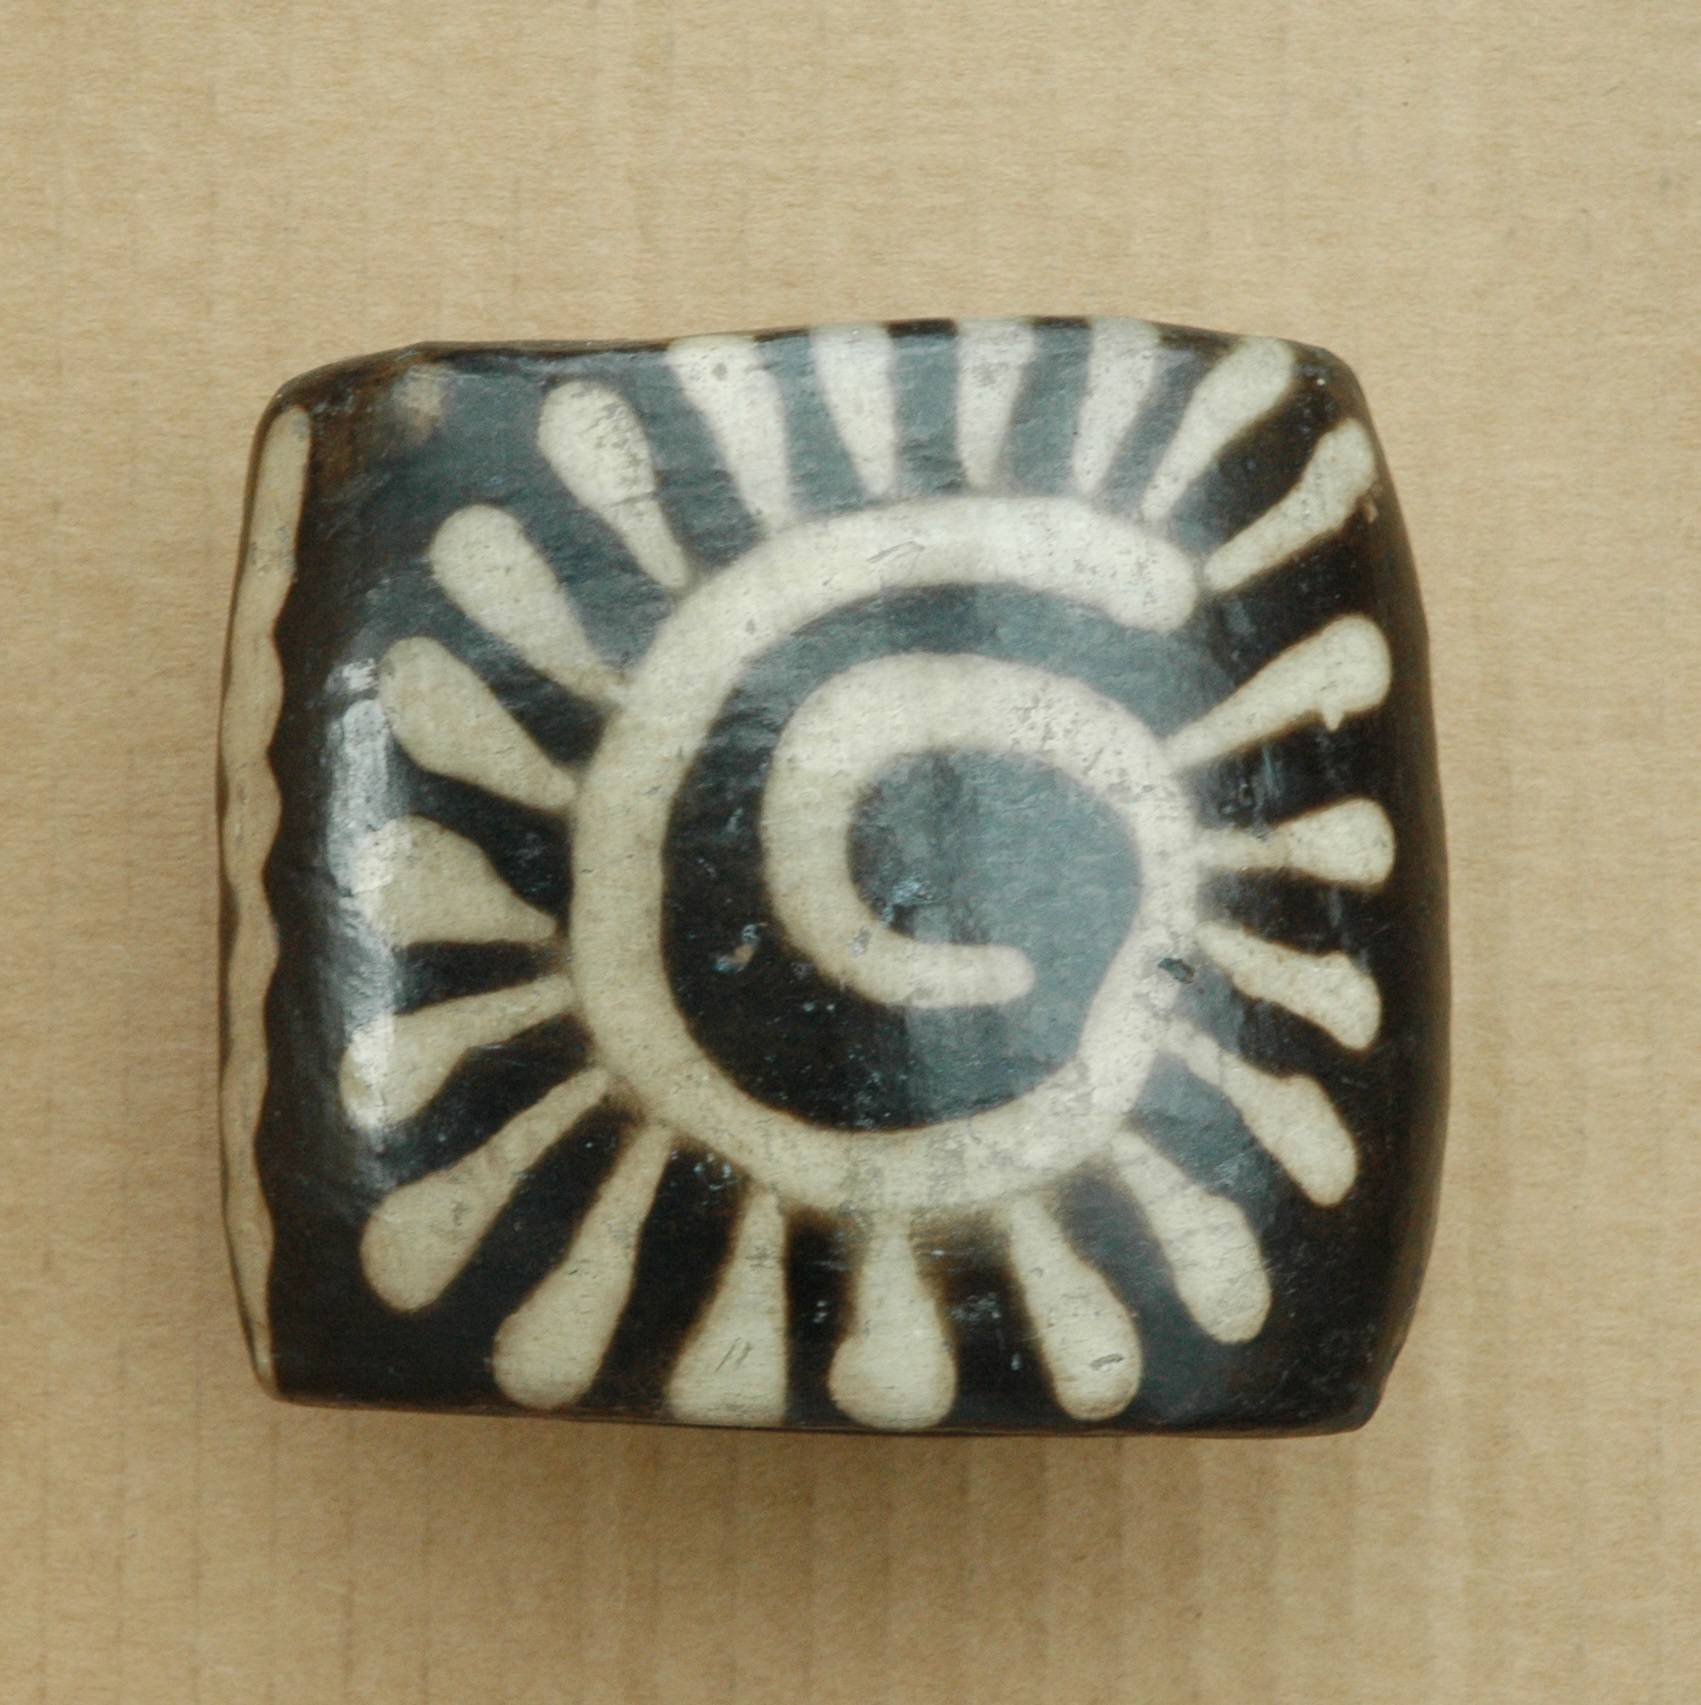
\includegraphics[width=0.15\textwidth]{interp/real_world_img/pot/pot}} &
\raisebox{-.5\height}{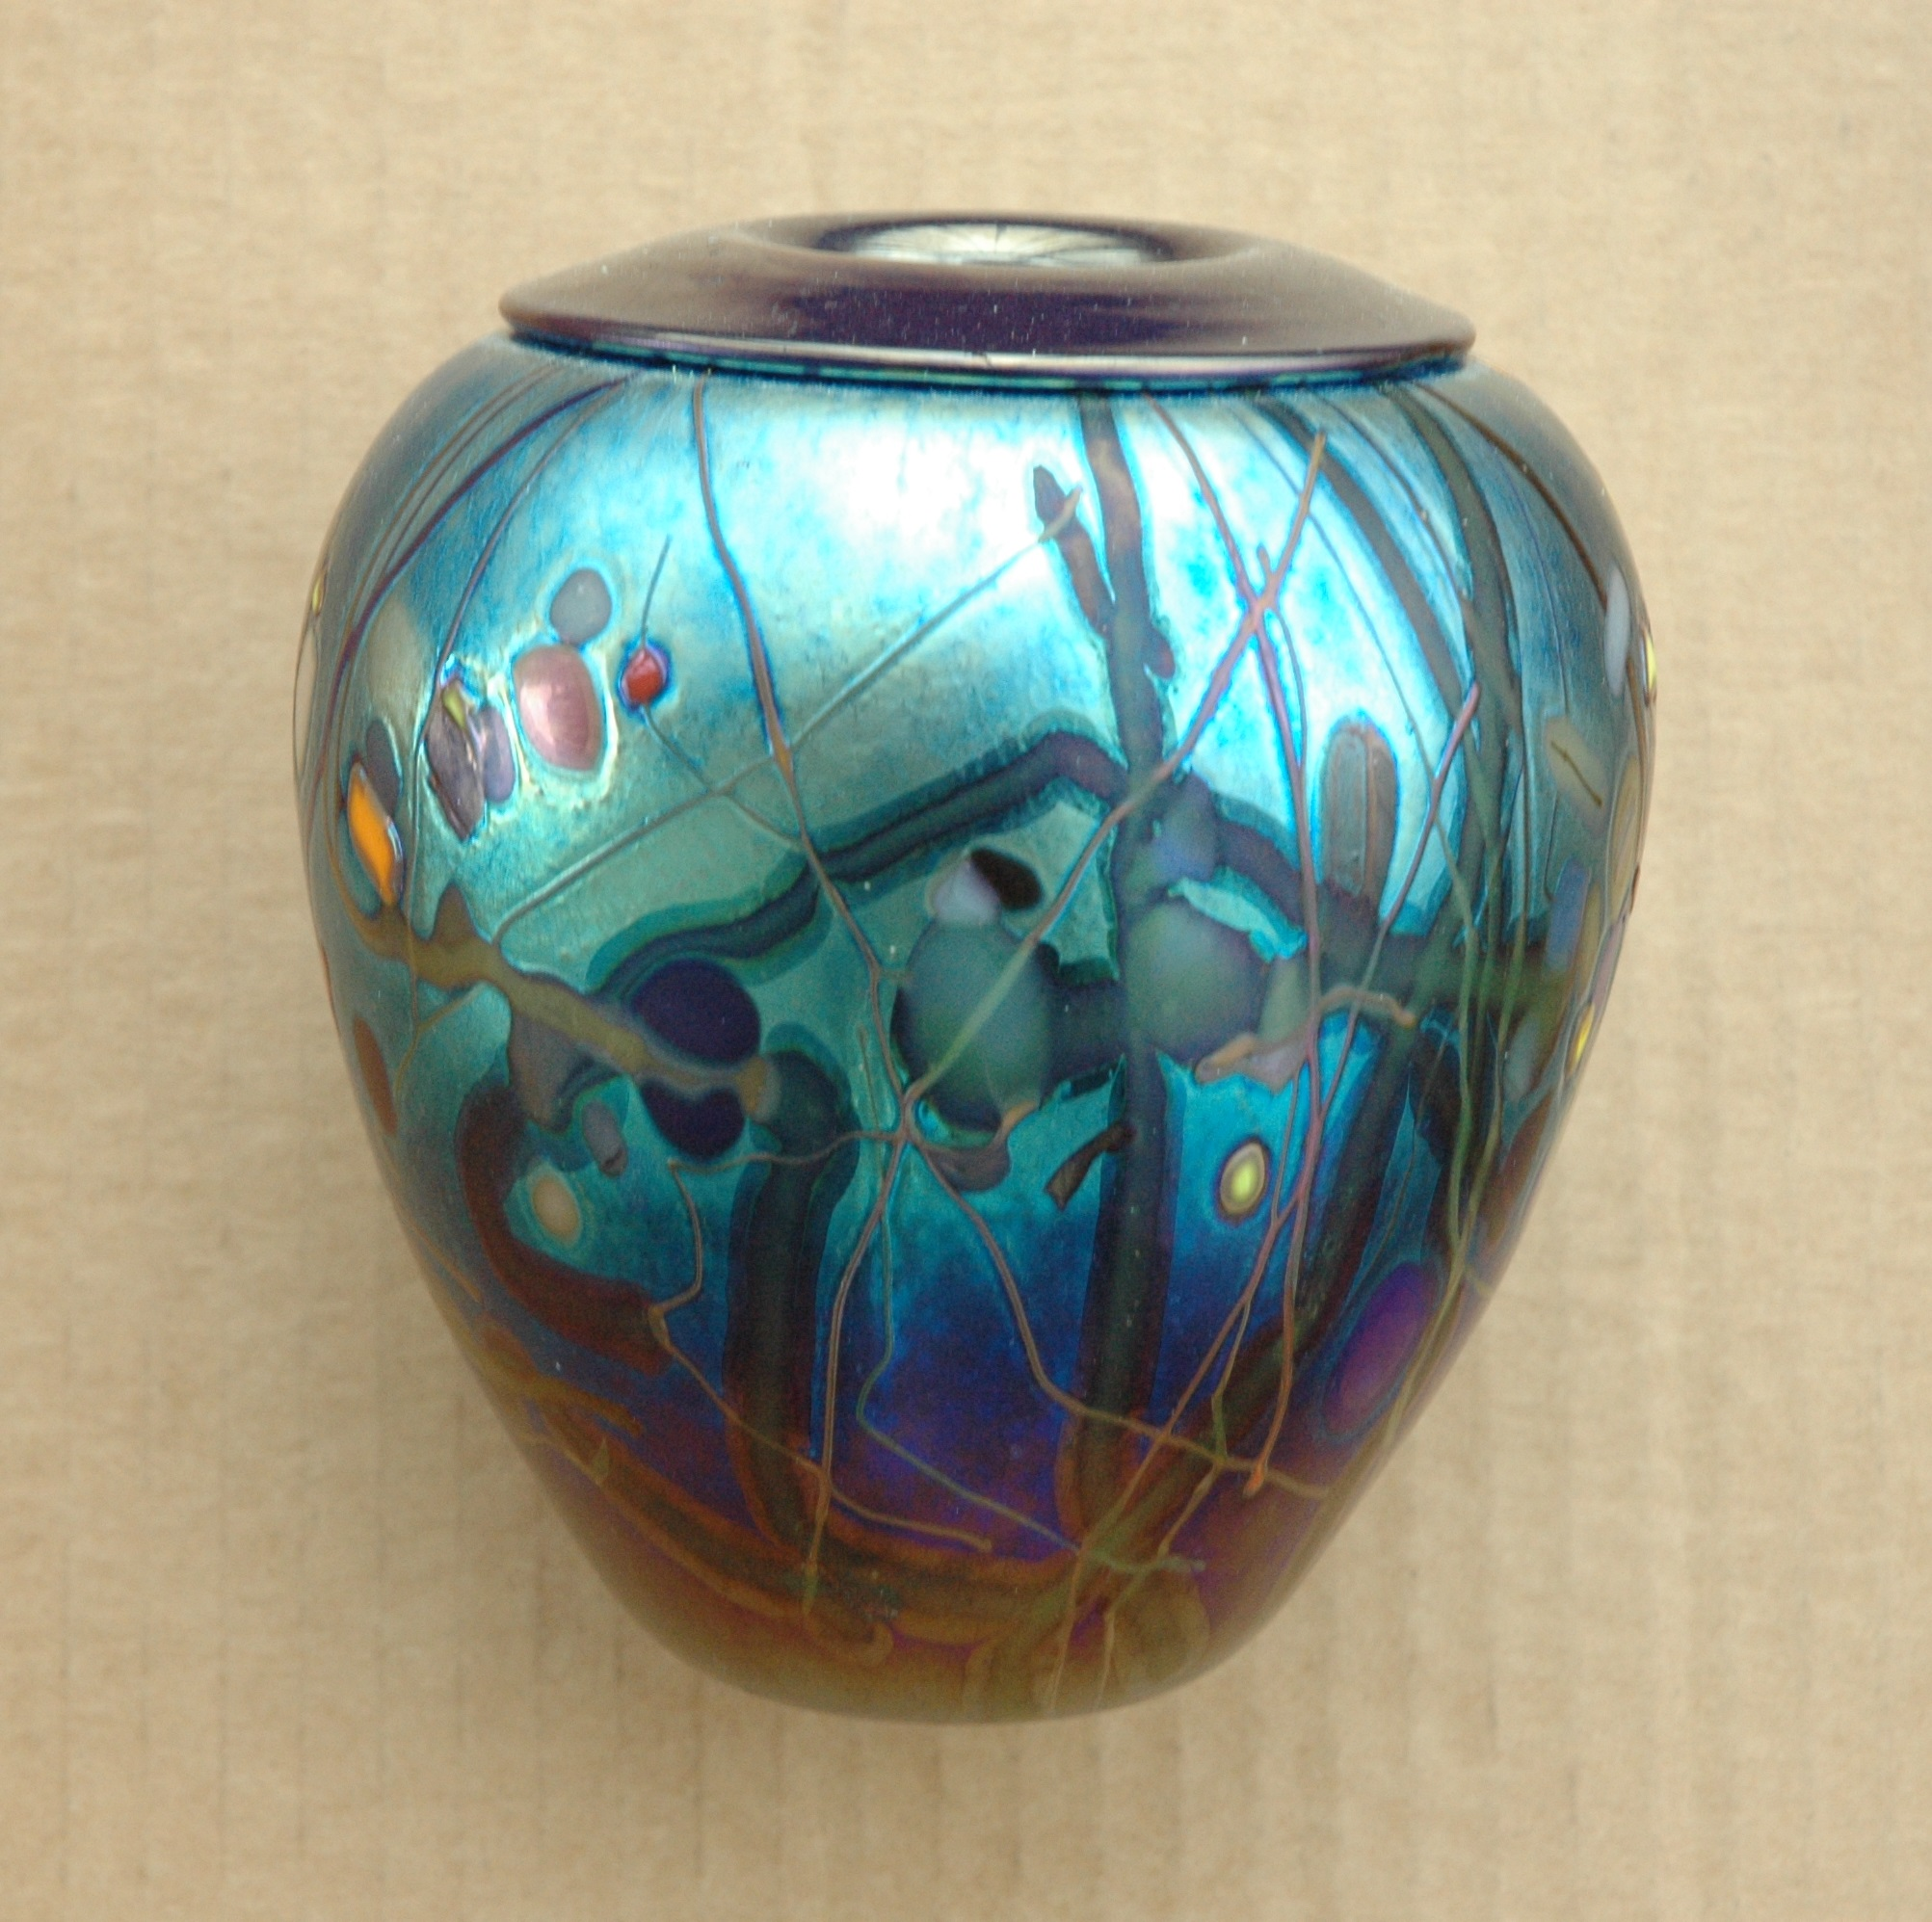
\includegraphics[width=0.15\textwidth]{interp/real_world_img/vase/vase}}\\ \cline{3-6}
\parbox[t]{2mm}{\multirow{3}{*}{\rotatebox[origin=c]{90}{Verbal}}}
& & \tabitem textureless & \tabitem textureless & \tabitem textured & \tabitem textured\\
& & \tabitem diffuse & \tabitem mixed d/s & \tabitem diffuse & \tabitem mixed d/s\\
& & \tabitem bright & \tabitem bright & \tabitem dark/bright & \tabitem dark/bright\\ \cline{3-6}
\parbox[t]{2mm}{\multirow{4}{*}{\rotatebox[origin=c]{90}{Description}}}
& Tex & 0.2 & 0.2 & 0.8 & 0.8\\
& Alb & 0.8 & 0.8 & 0.8 (0.2) & 0.8 (0.2)\\
& Spec & 0.2 & 0.8 & 0.2 & 0.8\\ % change from 0.5 to 0.8
& Rough & 0.8 & 0.2 & 0.2 & 0.2\\ \cline{3-6}
\parbox[t]{2mm}{\multirow{2}{*}{\rotatebox[origin=c]{90}{Alg}}}
& & \tabitem EPS & \tabitem \tc{EPS} & \tabitem PMVS & \tabitem\tc{PMVS} \\
& & \tabitem\tc{GSL} & \tabitem & \tabitem\tc{GSL} \\
\bottomrule
\end{tabular}
\caption{The repsentatives of the four classes of objects used for evaluation. Example images and problem conditions of real-world objects are in the first two rows. The correct description that matches the problem condition of corresponding object is presented in third row. The last row shows the algorithms returned by the mapping, from which the interpreter selects one successful algorithm, which is in colour red.}
\label{fig:real_data}
\end{figure}

\section{Evaluation of Interpreter}
\label{sec:eval_interp}
This section evaluates the proof of concept interpreter, which is three-fold: 1) given an accurate description, can the interpreter select an algorithm that achieves a successful reconstruction result; 2) given an less accurate description, would the interpreter perform poorer than given an accuracy; 3) given an inaccurate description, would the interpreter fail to achieve a successful reconstruction. We provide demonstrative results of the interpreter using the synthetic and real-world dataset, as shown in Figure~\ref{fig:synth_real_dataset}.

\subsection{Evaluation 1: accurate description, successful result}
In this section, we evaluate whether the interpreter can return a successful reconstruction result given a valid description of problem condition, see results in Figure~\ref{fig:eval_1}. The figure is divided into two sections, one for synthetic dataset and another for real-world dataset. The `Algo' row shows the algorithm selected by the interpreter, which also appear as the algorithm in red text in Figure~\ref{fig:synth_data},~\ref{fig:real_data}. The `Results' row shows the reconstruction results of the corresponding algorithm, and the `Baseline' row demonstrate the results of the baseline method. We utilize visual phenomena, such as surface roughness, holes, spikes as indicators of the reconstruction quality.

The baseline method achieves decent reconstruction results on all objects. Though due to the resolution of the voxel grids, the surfaces are relatively rough. Further, the surface concavities fail to be carved out for concave objects (Bust). The performance of the interpreter on both synthetic and real-world datasets are consistent in that the algorithms selected by the interpreter consistently outperform the baseline technique. All results have much smoother reconstructed surfaces, especially those of EPS and GSL, which is an indicator that the accuracy of the results are much higher using the selected algorithm. Further, erroneous results, such as surface holes, obtrutions, spikes are absent from the reconstruction results, which indicates that the selected algorithms can achieve completeness, and angular error no worse than the baseline.

Note that the selection of objects do no favor any algorithm. In fact, as we will show below, it is highly possible to get a poor result if another algorithm is chosen instead of the interpreted one. The significance of this study is that we demonstrated that it is achievable to translate a user-specified description, which has nothing to do with algorithm-level knowledge, to an algorithm selected from a suite of algorithms and achieve a successful reconstruction. There is no need to understand the underlying algorithms, or set the obscure algorithm specific parameters.
\begin{figure*}[!htbp]
\centering
\begin{tabular}{l|c|c|c|c}
\toprule
& \multicolumn{4}{c}{Synth-objects}\\ \cline{2-5}
& Bust & Vase0 & Barrel & Vase1\\
\midrule
\parbox[t]{2mm}{\rotatebox[origin=c]{90}{Algo}}
& GSL & EPS & GSL & PMVS \\
\parbox[t]{2mm}{\rotatebox[origin=c]{90}{Results}}
& \raisebox{-.5\height}{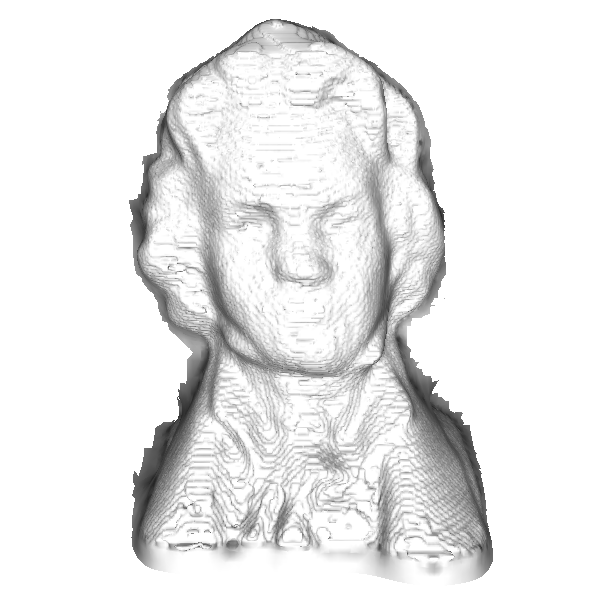
\includegraphics[width=0.15\textwidth]{interp/synth_interp/beethoven_sl}}
& \raisebox{-.5\height}{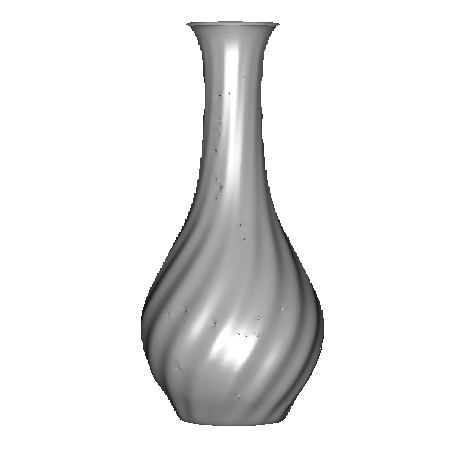
\includegraphics[width=0.15\textwidth]{interp/synth_interp/vase0_ps}}
& \raisebox{-.5\height}{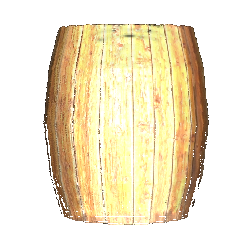
\includegraphics[width=0.15\textwidth]{interp/synth_interp/barrel_sl}}
& \raisebox{-.5\height}{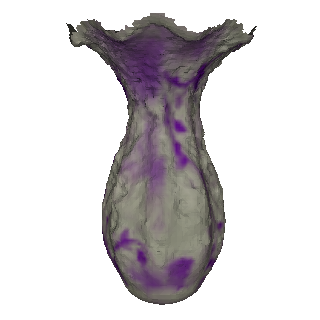
\includegraphics[width=0.15\textwidth]{interp/synth_interp/vase1_mvs}}\\
\parbox[t]{2mm}{\rotatebox[origin=c]{90}{Baseline}}
& \raisebox{-.5\height}{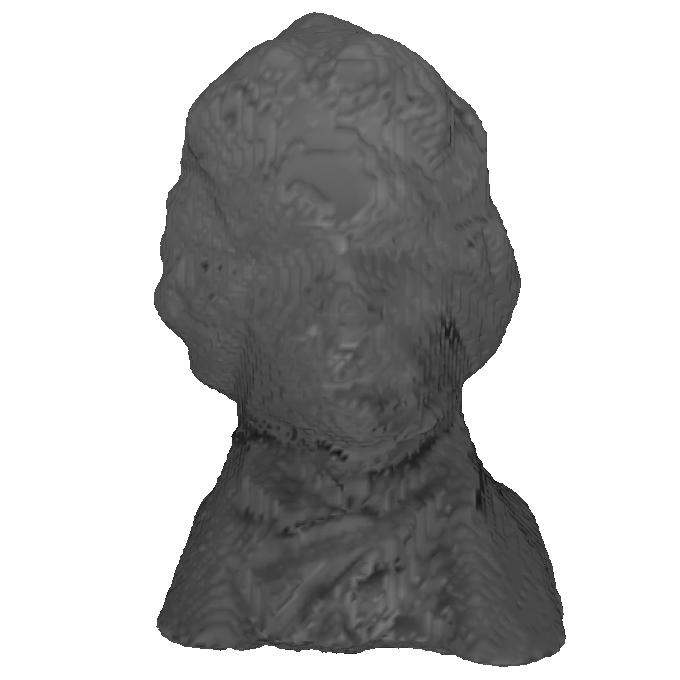
\includegraphics[width=0.15\textwidth]{interp/synth_interp/beethoven_vh}}
& \raisebox{-.5\height}{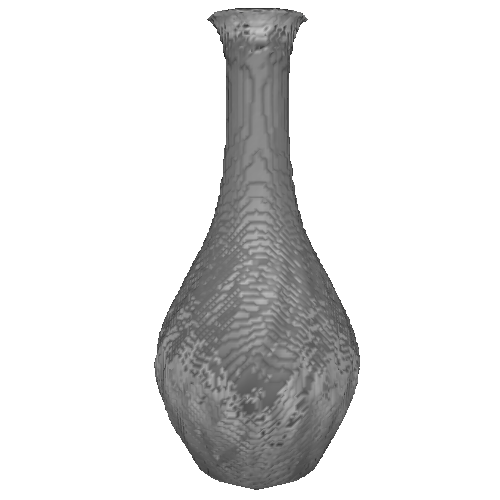
\includegraphics[width=0.15\textwidth]{interp/synth_interp/vase0_vh}}
& \raisebox{-.5\height}{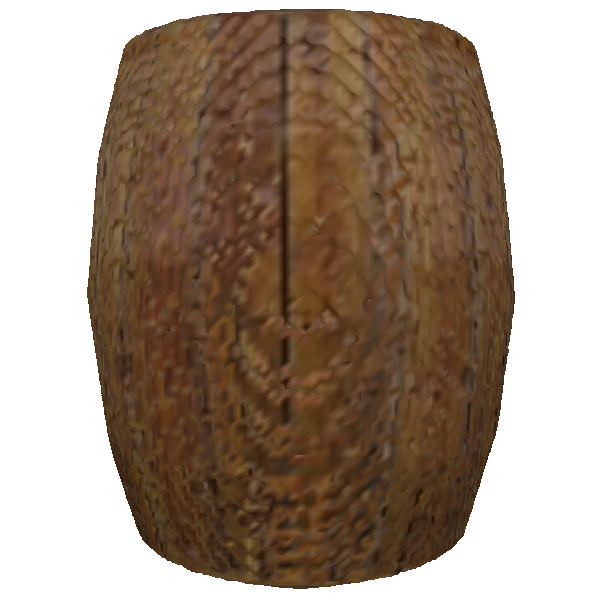
\includegraphics[width=0.15\textwidth]{interp/synth_interp/barrel_vh}}
& \raisebox{-.5\height}{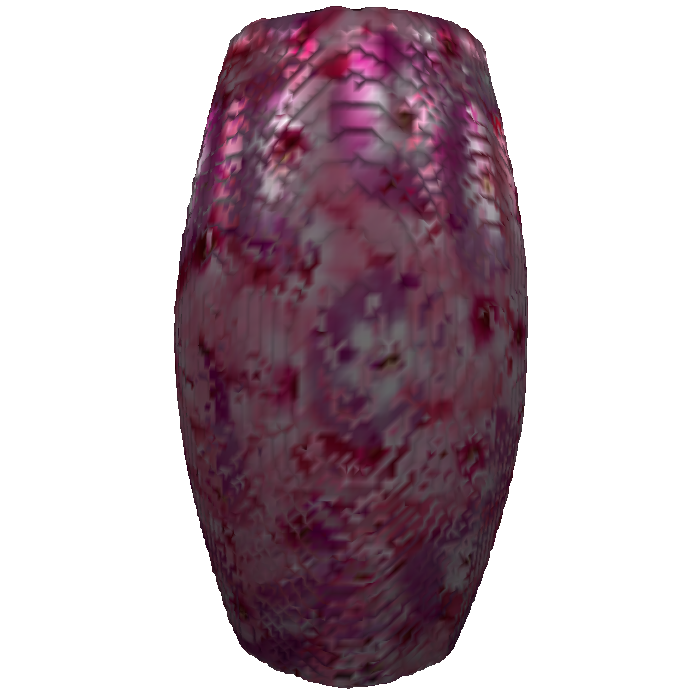
\includegraphics[width=0.15\textwidth]{interp/synth_interp/vase1_vh}}\\
\bottomrule
\toprule
& \multicolumn{4}{c}{Real-objects}\\ \cline{2-5}
& Statue & Cup & Pot & Vase \\
\midrule
\parbox[t]{2mm}{\rotatebox[origin=c]{90}{Algo.}}
& GSL & EPS & GSL & PMVS \\
\parbox[t]{2mm}{\rotatebox[origin=c]{90}{Results}}
& \raisebox{-.5\height}{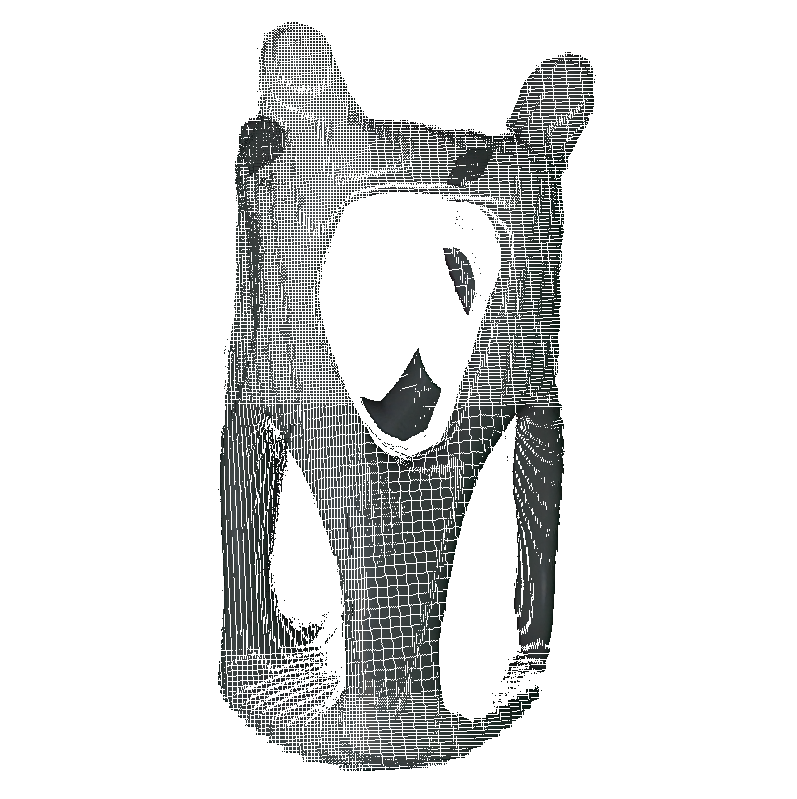
\includegraphics[width=0.15\textwidth]{interp/real_interp/statue/statue_sl}}
& \raisebox{-.5\height}{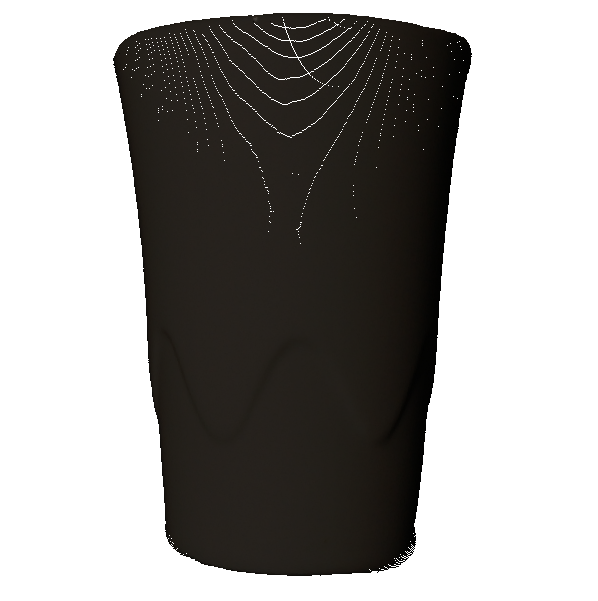
\includegraphics[width=0.15\textwidth]{interp/real_interp/cup/cup_ps}}
& \raisebox{-.5\height}{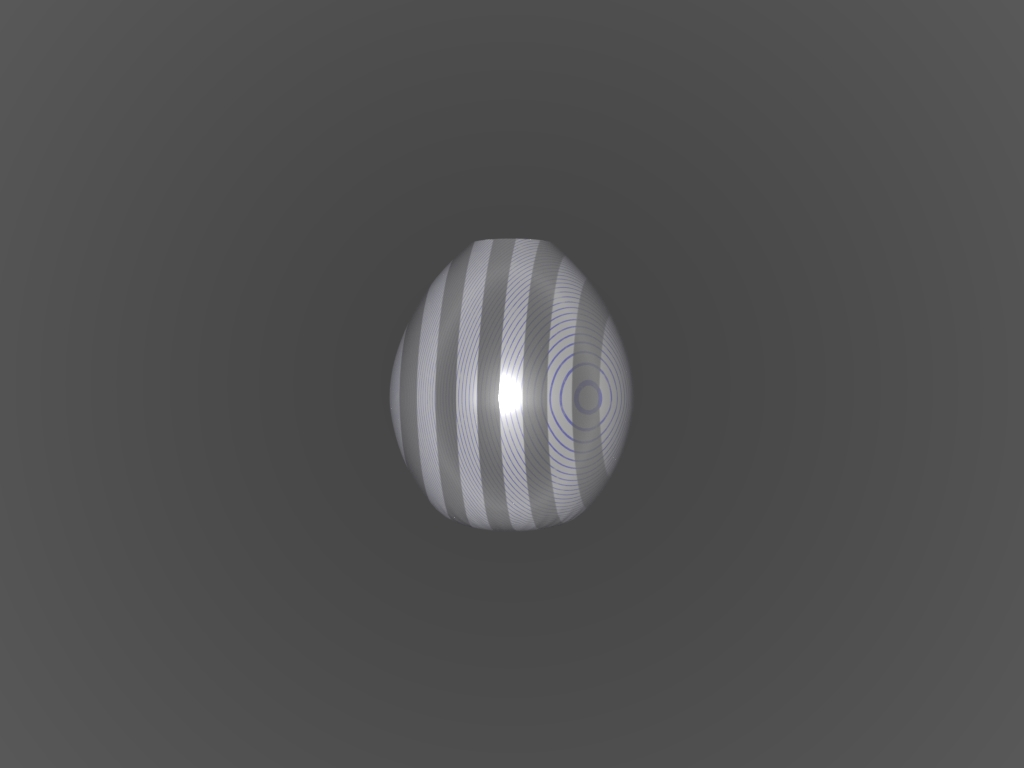
\includegraphics[width=0.15\textwidth]{interp/real_interp/pot/pot_sl}}
& \raisebox{-.5\height}{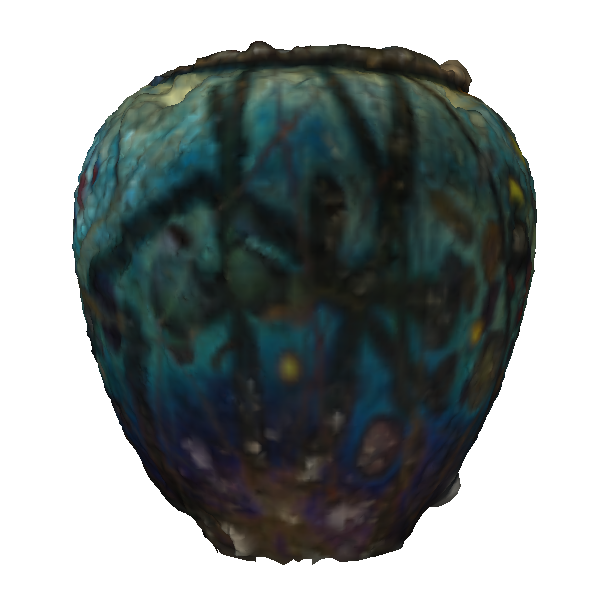
\includegraphics[width=0.15\textwidth]{interp/real_interp/vase/vase_mvs}}\\
\parbox[t]{2mm}{\rotatebox[origin=c]{90}{Baseline}}
& \raisebox{-.5\height}{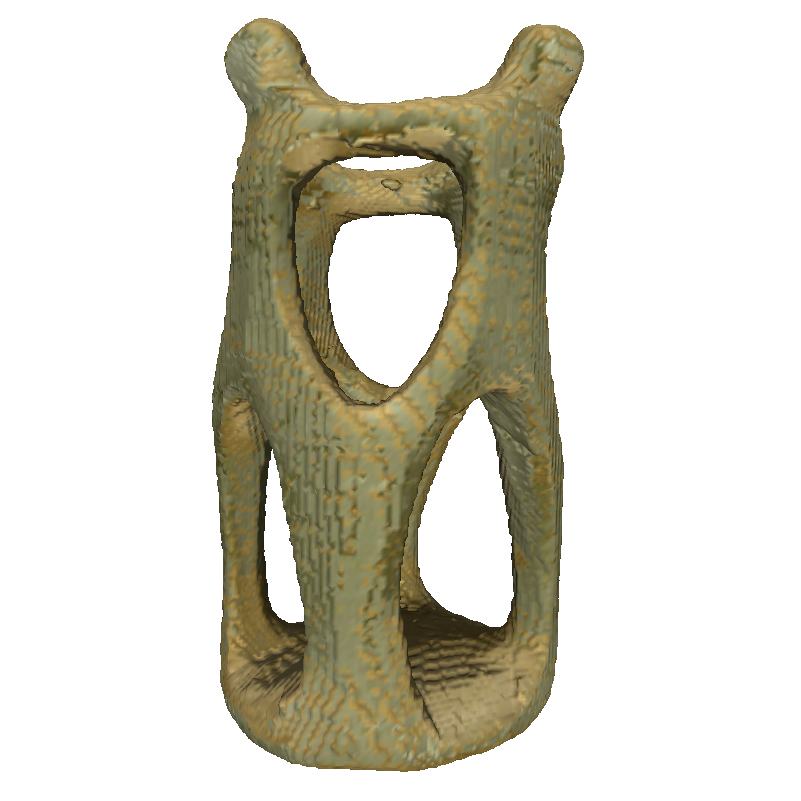
\includegraphics[width=0.15\textwidth]{interp/real_interp/statue/statue_sc}}
& \raisebox{-.5\height}{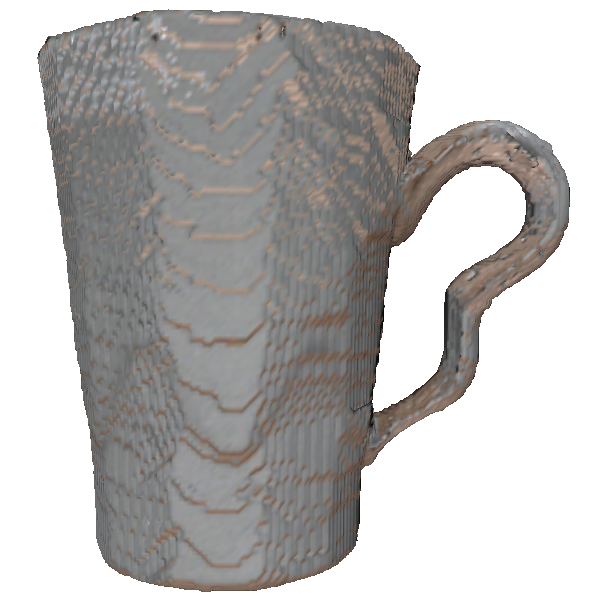
\includegraphics[width=0.15\textwidth]{interp/real_interp/cup/cup_sc}}
& \raisebox{-.5\height}{\includegraphics[width=0.15\textwidth]{interp/real_interp/pot/pot_sc}}
& \raisebox{-.5\height}{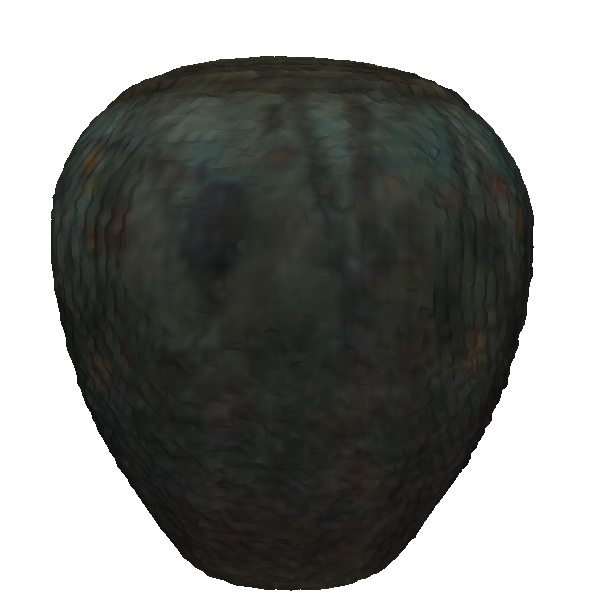
\includegraphics[width=0.15\textwidth]{interp/real_interp/vase/vase_sc}}\\
\bottomrule
\end{tabular}
\caption{Evaluation 1: correct description leads to successful reconstruction result. The baseline results are provided so that we can determine the quality of result returned by the algorithm chosen by the interpreter.}
\label{fig:eval_1}
\end{figure*}

\subsection{Evaluation 2: less accurate description, less successful result}
We have demonstrated in last section that the interpreter can achieve successful results given accurate description. However, how would the interpreter perform given an inaccurate description? There are two guesses: 1) the interpreter would return poor result given an inaccurate description; 2) the interpreter can still achieve successful results under some specific circumstances. In this section, we are interested to find out how sensitive the interpreter is given inaccurate descriptions, and the cases where it would fail or succeed. We provide four inaccurate desriptions by iterating through four properties, and each time one and only one property is set correctly. For instance, $\text{prop}_i$ is correctly estimated for $\text{desc}_i$ while the rest of the properties are set incorrectly, $i\in \{1, 2, 3, 4\}$. Since a description could be mapped to multiple algorithms, a description that does not match the object could potentially have a successful reconstruction result as well.

The layout of the graph is as follows: columnwise, $\text{Desc}_i, i\in\{1, 2, 3, 4\}$ presents results where an inaccurate description is provided while the last column presents the results where the correct description is provided. Rowwise, for each object, the result is divided into three segments: The description of problem condition is presented in the first segment, which is coloured-coded to indicate the correctly set property. The order of properties in the description is: texture, albedo, specularity, and roughness. Since there is one and only one correctly estimated property in each inaccurate description, it is coloured in red while the incorrectly estimated properties are coloured in black. The algorithms returned by the mapping are presented below the description in the second segment, with the algorithm chosen by the interpreter coloured in red. The reconstruction result using the interpreted algorithm is shown in the last segment of each section.
\begin{figure*}[!htbp]
\centering
\begin{tabular}{c|*{4}{l}|l}
\toprule
\multirow{2}{*}{Object} & \multicolumn{5}{c}{Descriptions and Results} \\ \cline{2-6}
& $Desc_1$ & $Desc_2$ & $Desc_3$ & $Desc_4$ & Correct Desc \\
\midrule
\multirow{4}{*}{Bust} & \tc{02}020802 & 08\tc{08}0802 & 0802\tc{02}02 & 080208\tc{08} & 02080208 \\
& \tabitem\tc{BL} & \tabitem PMVS 	 & \tabitem\tc{PMVS} & \tabitem\tc{EPS} & \tabitem EPS 	  \\
& 		 		  & \tabitem EPS  	 & 	    	 		 & 	 			  	& \tabitem\tc{GSL}\\
& 		 		  & \tabitem\tc{GSL} & 	    	 		 & 	 			  	& 				  \\
& 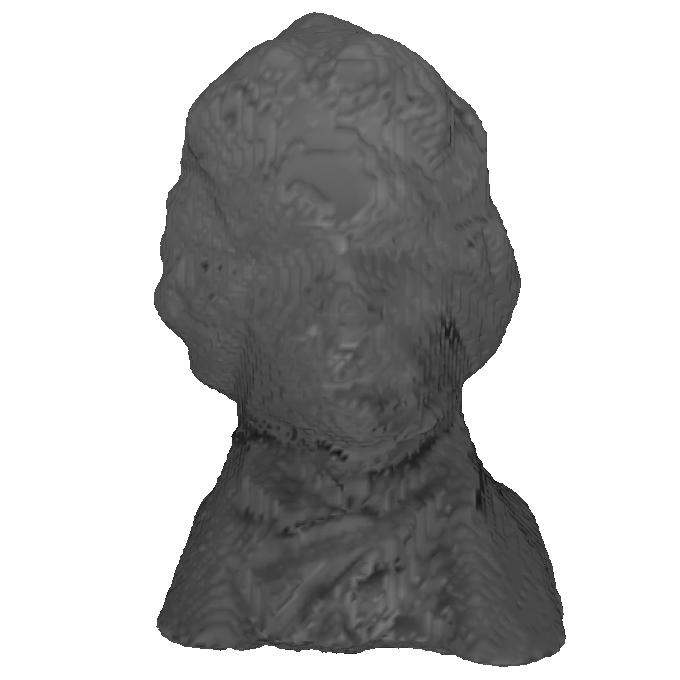
\includegraphics[width=0.1\textwidth]{interp/synth_interp/beethoven_vh} &
  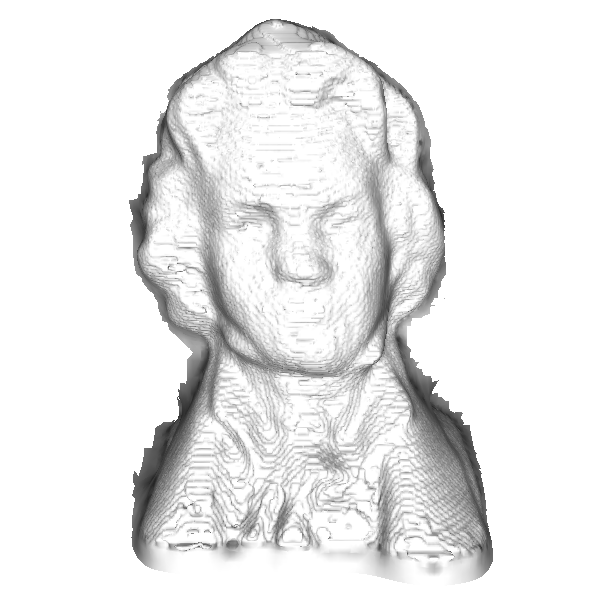
\includegraphics[width=0.1\textwidth]{interp/synth_interp/beethoven_sl} &
  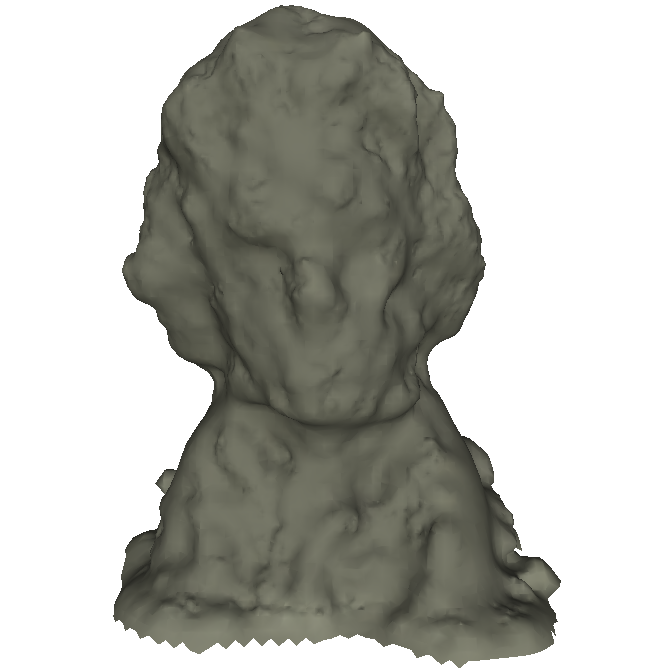
\includegraphics[width=0.1\textwidth]{interp/synth_interp/beethoven_mvs} &
  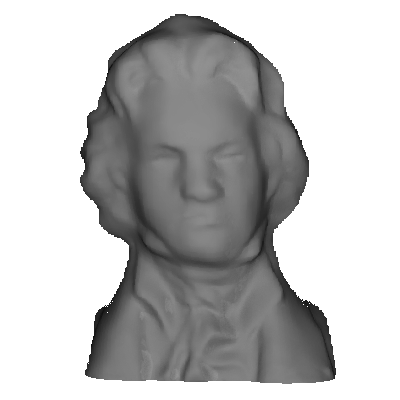
\includegraphics[width=0.1\textwidth]{interp/synth_interp/beethoven_ps} &
  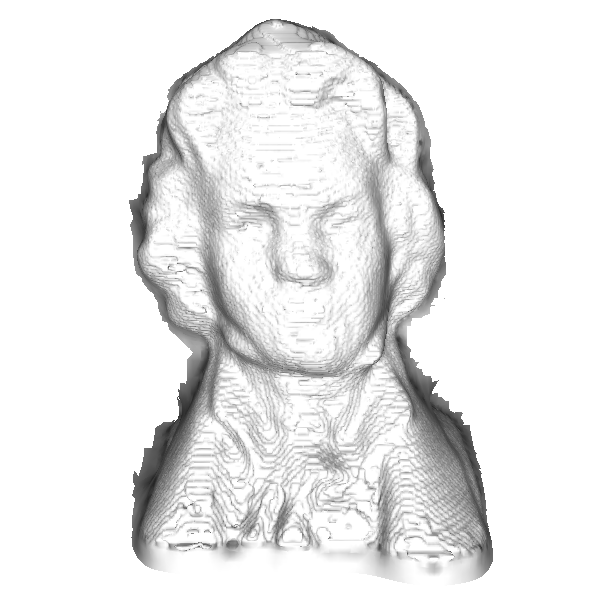
\includegraphics[width=0.1\textwidth]{interp/synth_interp/beethoven_sl} \\ \cline{2-6}
\multirow{4}{*}{vase0} & \tc{02}080208 & 08\tc{08}0208 & 0802\tc{08}02 & 080202\tc{02} & 02080802 \\
& \tabitem EPS 	   & \tabitem PMVS   & \tabitem\tc{BL} & \tabitem\tc{PMVS} & \tabitem\tc{EPS}\\
& \tabitem\tc{GSL} & \tabitem EPS 	 & 				   & 				   &\\
& 			   	   & \tabitem\tc{GSL}& 				   & 				   &\\
& \includegraphics[width=0.1\textwidth]{interp/synth_interp/vase0_sl} &
  \includegraphics[width=0.1\textwidth]{interp/synth_interp/vase0_sl} &
  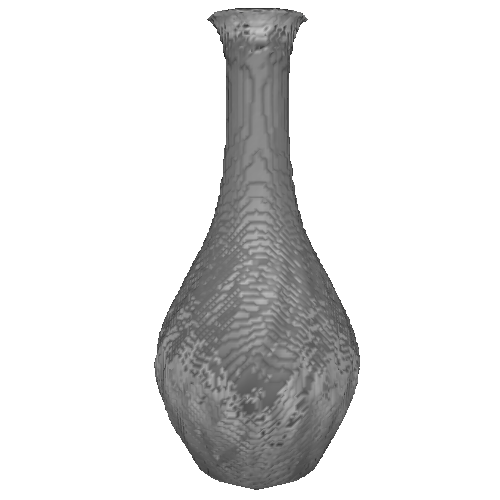
\includegraphics[width=0.1\textwidth]{interp/synth_interp/vase0_vh} &
  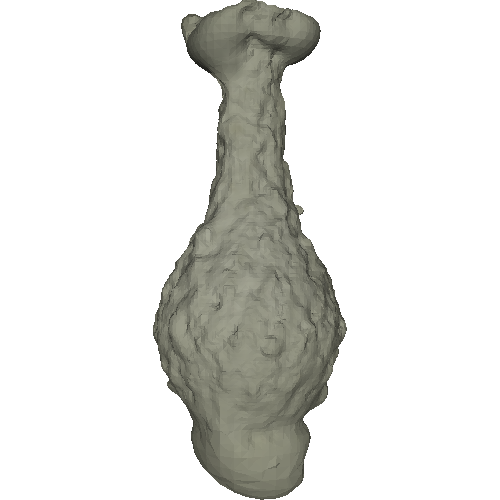
\includegraphics[width=0.1\textwidth]{interp/synth_interp/vase0_mvs} &
  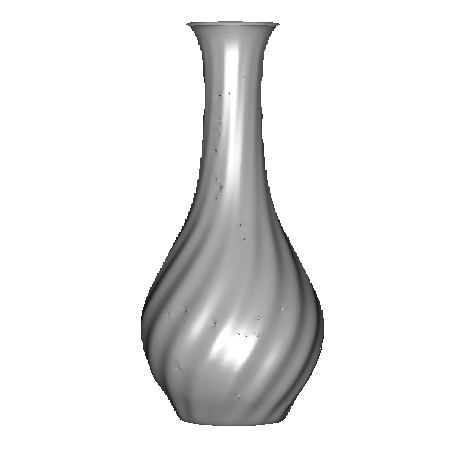
\includegraphics[width=0.1\textwidth]{interp/synth_interp/vase0_ps} \\ \cline{2-6}
\multirow{4}{*}{barrel} & \tc{08}020802 & 02\tc{08}0802 & 0202\tc{02}02 & 020208\tc{08} & 08080208 \\
& \tabitem\tc{PMVS} & \tabitem EPS     & \tabitem\tc{BL} & \tabitem\tc{EPS} & \tabitem PMVS   \\
& 					& \tabitem\tc{GSL} & 				 & 					& \tabitem EPS    \\
& 					& 				   & 				 &					& \tabitem\tc{GSL}\\
& 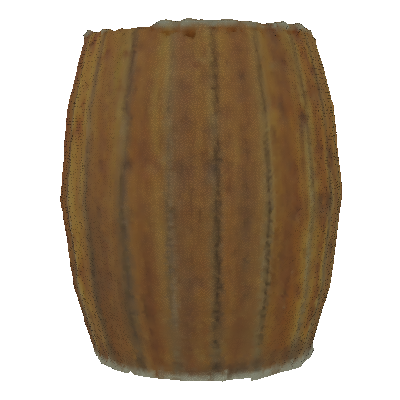
\includegraphics[width=0.1\textwidth]{interp/synth_interp/barrel_mvs} &
  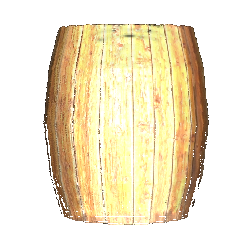
\includegraphics[width=0.1\textwidth]{interp/synth_interp/barrel_sl} &
  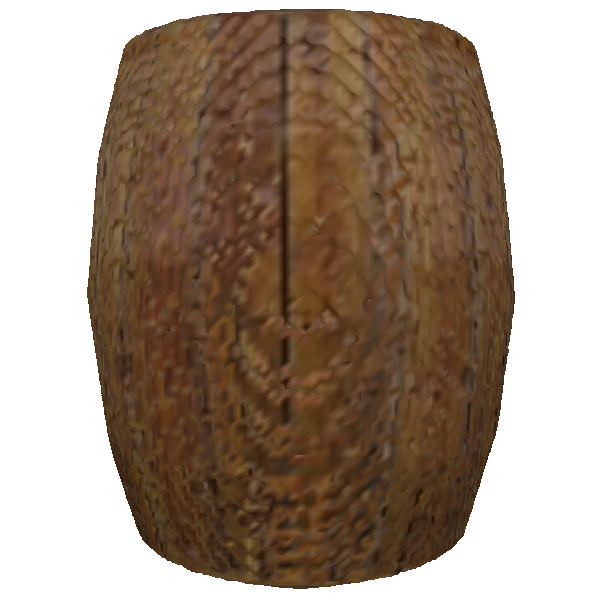
\includegraphics[width=0.1\textwidth]{interp/synth_interp/barrel_vh} &
  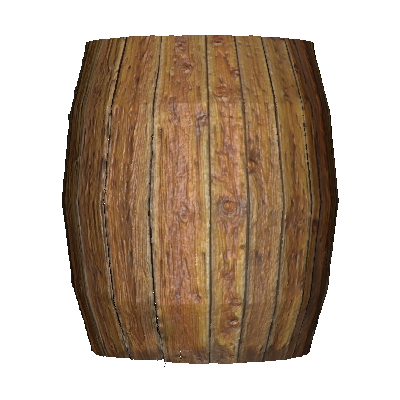
\includegraphics[width=0.1\textwidth]{interp/synth_interp/barrel_ps} &
  \includegraphics[width=0.1\textwidth]{interp/synth_interp/barrel_sl} \\ \cline{2-6}
\multirow{4}{*}{vase1} & \tc{08}020208 & 02\tc{08}0208 & 0202\tc{08}08 & 020202\tc{02} & 08080802 \\
& \tabitem\tc{PMVS} & \tabitem EPS     & \tabitem\tc{BL} & \tabitem\tc{BL} & \tabitem\tc{PMVS}\\
& \tabitem EPS 		& \tabitem\tc{GSL} &				 &				   & \tabitem EPS     \\
& \includegraphics[width=0.1\textwidth]{interp/synth_interp/vase1_mvs} &
  \includegraphics[width=0.1\textwidth]{interp/synth_interp/vase1_sl} &
  \includegraphics[width=0.1\textwidth]{interp/synth_interp/vase1_vh} &
  \includegraphics[width=0.1\textwidth]{interp/synth_interp/vase1_vh} &
  \includegraphics[width=0.1\textwidth]{interp/synth_interp/vase1_mvs}\\
\bottomrule
\end{tabular}
\caption{Evaluation 2: less accurate description may lead to poor result. $\text{Desc}_i$ represents inaccurate descriptions. For each object, the first row represent the description, with the correctly estimated property coloured in red while the incorrect ones in black. The algorithms determined by mapping are below the description with the algorithm selected by interpreter coloured in red (BL: baseline). The last row shows the corresponding reconstruction results.}
\label{fig:eval_21}
\end{figure*}

\begin{figure*}[!htbp]
\centering
\begin{tabular}{c|*{4}{l}|l}
\toprule
\multirow{2}{*}{Object} & \multicolumn{5}{c}{Descriptions and Results} \\ \cline{2-6}
& $Desc_1$ & $Desc_2$ & $Desc_3$ & $Desc_4$ & Correct Desc \\
\midrule
\multirow{4}{*}{statue} & \tc{02}020802 & 08\tc{08}0802 & 0802\tc{02}02 & 080208\tc{08} & 02080208 \\
& \tabitem\tc{BL} & \tabitem PMVS 	 & \tabitem\tc{PMVS} & \tabitem\tc{EPS} & \tabitem EPS 	  \\
& 		 		  & \tabitem EPS  	 & 	    	 		 & 	 			  	& \tabitem\tc{GSL}\\
& 		 		  & \tabitem\tc{GSL} & 	    	 		 & 	 			  	&\\
& \includegraphics[width=0.1\textwidth]{interp/real_interp/statue/statue_sc} &
  \includegraphics[width=0.1\textwidth]{interp/real_interp/statue/statue_sl} &
  \includegraphics[width=0.1\textwidth]{interp/real_interp/statue/statue_mvs} &
  \includegraphics[width=0.1\textwidth]{interp/real_interp/statue/statue_ps} &
  \includegraphics[width=0.1\textwidth]{interp/real_interp/statue/statue_sl} \\ \cline{2-6}
\multirow{4}{*}{cup} & \tc{02}080208 & 08\tc{08}0208 & 0802\tc{08}02 & 080202\tc{02} & 02080802 \\
& \tabitem EPS 	   & \tabitem PMVS   & \tabitem\tc{BL} & \tabitem\tc{PMVS} & \tabitem\tc{EPS}\\
& \tabitem\tc{GSL} & \tabitem EPS 	 & 				   & \\
& 			   	   & \tabitem\tc{GSL}& 				   & 				   &\\
& \includegraphics[width=0.1\textwidth]{interp/real_interp/cup/cup_sl} &
  \includegraphics[width=0.1\textwidth]{interp/real_interp/cup/cup_sl} &
  \includegraphics[width=0.1\textwidth]{interp/real_interp/cup/cup_sc} &
  \includegraphics[width=0.1\textwidth]{interp/real_interp/cup/cup_mvs} &
  \includegraphics[width=0.1\textwidth]{interp/real_interp/cup/cup_ps} \\ \cline{2-6}
\multirow{4}{*}{pot} & \tc{08}020802 & 02\tc{08}0802 & 0202\tc{02}02 & 020208\tc{08} & 08080208 \\
& \tabitem\tc{PMVS} & \tabitem EPS     & \tabitem\tc{BL} & \tabitem\tc{EPS} & \tabitem PMVS   \\
& 					& \tabitem\tc{GSL} & 				 & 					& \tabitem EPS    \\
& 					& 				   & 				 &					& \tabitem\tc{GSL}\\
& \includegraphics[width=0.1\textwidth]{interp/real_interp/pot/pot_mvs} &
  \includegraphics[width=0.1\textwidth]{interp/real_interp/pot/pot_sl} &
  \includegraphics[width=0.1\textwidth]{interp/real_interp/pot/pot_sc} &
  \includegraphics[width=0.1\textwidth]{interp/real_interp/pot/pot_ps} &
  \includegraphics[width=0.1\textwidth]{interp/real_interp/pot/pot_sl} \\ \cline{2-6}
\multirow{4}{*}{vase} & \tc{08}020208 & 02\tc{08}0208 & 0202\tc{08}08 & 020202\tc{02} & 08080802 \\
& \tabitem\tc{PMVS} & \tabitem EPS     & \tabitem\tc{BL} & \tabitem\tc{BL} & \tabitem\tc{PMVS}\\
& \tabitem EPS 		& \tabitem\tc{GSL} &				 &				   & \tabitem EPS     \\
& \includegraphics[width=0.1\textwidth]{interp/real_interp/vase/vase_mvs} &
  \includegraphics[width=0.1\textwidth]{interp/real_interp/vase/vase_sl} &
  \includegraphics[width=0.1\textwidth]{interp/real_interp/vase/vase_sc} &
  \includegraphics[width=0.1\textwidth]{interp/real_interp/vase/vase_sc} &
  \includegraphics[width=0.1\textwidth]{interp/real_interp/vase/vase_mvs}\\
\bottomrule
\end{tabular}
\caption{Evaluation 2: less accurate description may lead to poor reconstruction results. $\text{Desc}_i$ represents inaccurate descriptions. For each object, the first row represent the description, with the correctly estimated property coloured in red while the incorrect ones in black. The algorithms determined by mapping are below the description with the algorithm selected by interpreter coloured in red (BL: baseline). The last row shows the corresponding reconstruction results.}
\label{fig:eval_22}
\end{figure*}
% paraphrase this: We can see that inaccurate description can lead to poor reconstruction, and it leads to successful results only when the selected algorithm is in the mapping of the correct description.

Let's denote the algorithm(s) returned by the mapping given description $\text{Desc}_i$ as $\{\text{Algo}_i\}$. For instance, the algorithms for object \textit{bust} given description $\text{Desc}_2$ is $\text{Algo}_2=\{PMVS, EPS, GSL\}$. Let's also denote the algorithm(s) returned by the correct description as $\{\text{Algo}\}$. Thus in the case of object \textit{bust}, $\{\text{Algo}\}=\{EPS, GSL\}$. We observe that an inaccurate description can possibly lead to a successful reconstruction if and only if 
$$
\{\text{Algo}_i\} \bigcap \{\text{Algo}\} \neq \emptyset
$$

The reason is that there are multiple algorithms that could work successfully for a specific object. Thus if an algorithm other than the interpreted one is chosen given an inaccurate description, a successful reconstruction result is still achievable. Let's use \textit{bust} as an example, $\text{Desc}_1$ and $\text{Desc}_3$ lead to poor results whereas $\text{Desc}_2$ and $\text{Desc}_4$ result in successful reconstructions. We can see that neither $\text{Desc}_1$ nor $\text{Desc}_3$ is mapped to any algorithm that is in common with those returned given accurate description. Further, both $\text{Desc}_2$ and $\text{Desc}_4$ have at least one mapped algorithm that coincides with the algorithms returned given accurate description. The take-away message is that for an incorrect description, the reconstruction results are generally worse than that of the interpreted result. However, for conditions that have multiple working algorithms, there may very well be an acceptable result.

\subsection{Evaluation 3: inaccurate description, poor result}
We have demonstrated that given a less accurate description, the results may or may not be poor. In cases where the algorithms mapped from inaccurate description coincide with algorithms returned from accurate description, it is still possible to achieve successful reconstruction. In this section, we are interested to see if this conclusion can also be applied to complete inaccurate description, \ie is it still possible to return a successful result. In this section, we evaluate whether the interpreter would return a poor reconstruction result given an inaccurate description of problem condition. We evaluate the performance of the interpreter using both synthetic and real-world objects.
\begin{figure*}[!htbp]
\centering
\begin{tabular}{c|*{4}{l}}
\toprule
Object & Bust & Vase0 & Barrel & Vase1 \\
\midrule
\parbox[t]{2mm}{\multirow{4}{*}{\rotatebox[origin=c]{90}{Incorrect Desc}}} 
& 08020802 & 08020208 & 02020802 & 02020208 \\
& \tabitem\tc{BL} & \tabitem\tc{PMVS} & \tabitem\tc{BL} & \tabitem\tc{EPS} \\
& 				  & \tabitem EPS \\
& \includegraphics[width=0.1\textwidth]{interp/synth_interp/beethoven_vh}
& \includegraphics[width=0.1\textwidth]{interp/synth_interp/vase0_mvs}
& \includegraphics[width=0.1\textwidth]{interp/synth_interp/barrel_vh}
& \includegraphics[width=0.1\textwidth]{interp/synth_interp/vase1_ps} \\ \cline{2-5}
\parbox[t]{2mm}{\multirow{5}{*}{\rotatebox[origin=c]{90}{Correct Desc}}}
& 02080208 & 02080802 & 08080208 & 08080802 \\
& \tabitem EPS 		& \tabitem\tc{EPS} & \tabitem PMVS 		& \tabitem\tc{PMVS} \\
& \tabitem\tc{GSL} 	&				   & \tabitem EPS  		& \tabitem EPS \\
& 					& 				   & \tabitem\tc{GSL}	& \\
& \includegraphics[width=0.1\textwidth]{interp/synth_interp/beethoven_sl}
& \includegraphics[width=0.1\textwidth]{interp/synth_interp/vase0_ps}
& \includegraphics[width=0.1\textwidth]{interp/synth_interp/barrel_sl}
& \includegraphics[width=0.1\textwidth]{interp/synth_interp/vase1_mvs} \\
\bottomrule
\toprule
Object & Statue & Cup & Pot & Vase \\
\midrule
\parbox[t]{2mm}{\multirow{4}{*}{\rotatebox[origin=c]{90}{Incorrect Desc}}}
& 08020802 & 08020208 & 02020802 & 02020208 \\
& \tabitem\tc{BL} & \tabitem\tc{PMVS} & \tabitem\tc{BL} & \tabitem\tc{EPS} \\
& 				  & \tabitem EPS \\
& \includegraphics[width=0.1\textwidth]{interp/real_interp/statue/statue_sc}
& \includegraphics[width=0.1\textwidth]{interp/real_interp/cup/cup_mvs}
& \includegraphics[width=0.1\textwidth]{interp/real_interp/pot/pot_sc}
& \includegraphics[width=0.1\textwidth]{interp/real_interp/vase/vase_ps} \\ \cline{2-5}
\parbox[t]{2mm}{\multirow{5}{*}{\rotatebox[origin=c]{90}{Correct Desc}}}
& 02080208 & 02080802 & 08080208 & 08080802 \\
& \tabitem EPS 		& \tabitem\tc{EPS} & \tabitem PMVS 		& \tabitem\tc{PMVS} \\
& \tabitem\tc{GSL} 	&				   & \tabitem EPS  		& \tabitem EPS \\
& 					& 				   & \tabitem\tc{GSL}	& \\
& \includegraphics[width=0.1\textwidth]{interp/real_interp/statue/statue_sl}
& \includegraphics[width=0.1\textwidth]{interp/real_interp/cup/cup_ps}
& \includegraphics[width=0.1\textwidth]{interp/real_interp/pot/pot_sl}
& \includegraphics[width=0.1\textwidth]{interp/real_interp/vase/vase_mvs} \\
\bottomrule
\end{tabular}
\caption{Evaluation 3: inaccurate description may lead to poor result. For each description, the first row represent the settins of properties. The algorithms determined by mapping are shown below with the algorithm selected by interpreter coloured in red (BL: baseline). The last row shows the corresponding reconstruction results. We can see that the results of inaccurate descriptions are poorer then those of accurate descriptions.}
\label{fig:eval_3}
\end{figure*}

The figure is divided into two sections: one for inaccurate description and one for accurate description. The inaccurate description is property-wise opposite to the corresponding accurate description. The mapped algorithms are shown below the description, with the algorithm chosen by the interpreter coloured in red. The reconstruction result by the interpreted algorithm is shown as well.

From the study of less accurate desription, we have already found out that it is still possible to achieve a successful result given an inaccurate description. However, it becomes more challenging, and more likely to select a less successful algorithm or the baseline method. There is a certain limit to the tolerance of inaccuracy of property estimation. Thus, the take-away message is that the interpreter, in some cases, can still performs reliably given an inaccurate description. However, it becomes more likely to fail to achieve a successful result given an completely inaccurate description of problem condition.

% \subsubsection{Description 1: Bust}
% Description 1 matches with object \textit{bust}, thus the algorithm selected by the interpreter achieves successful reconstruction result. The problem condition of object \textit{barrel} is also mapped to algorithm GSL, that is why the reconstruction result of \textit{barrel} is also successful.

% \subsubsection{Description 2: Vase0}
% Description 2 matches with object \textit{vase0}, thus the algorithm selected by the interpreter achieves successful reconstruction result. The problem condition of all objects mapped to EPS, that is why the all reconstruction results by EPS are successful.

% \subsubsection{Description 3: Barrel}
% Description 3 matches with object \textit{barrel}, which has a reliable reconstruction result. The selected algorithm GSL is also in the mapped algorithms of object \textit{bust}, as shown in Table~\ref{tab:synth_prop_list}. Thus even though \textbf{description 3} doesn't match with the problem condition of \textit{bust}, a satisfactory result is also returned. However, the selected algorithm is not in the mapped algorithms of object \textit{vase0} and \textit{vase1}, thus less successful results are returned.

% \subsubsection{Description 4: Vase1}
% Description 4 matches with object \textit{vase1}, thus the algorithm selected by the interpreter achieves successful reconstruction result. The problem condition of object \textit{barrel} is also mapped to algorithm PMVS, that is why the reconstruction result of \textit{barrel} is also successful.

% \subsubsection{Description 1: statue}
% Description 1 matches with object \textit{statue}, thus the algorithm selected by the interpreter achieves successful reconstruction result. The problem condition of object \textit{cup} and \textit{pot} are also mapped to algorithm GSL, that is why the reconstruction result of these two objects are also successful.

% \subsubsection{Description 2: cup}
% Description 2 matches with object \textit{cup}, thus the algorithm selected by the interpreter achieves successful reconstruction result. The problem condition of \textit{statue} is mapped to EPS, that is why the all reconstruction result of \textit{statue} by EPS is successful.

% \subsubsection{Description 3: pot}
% Description 3 matches partially with object \textit{pot} since it has both high and low albedo surface areas. The surface area with high albedo is well reconstructed whereas the surface with low albedo, which doesn't match the description is not reconstructed at all. The selected algorithm is also in the mapped algorithms of object \textit{statue} and \textit{cup}, thus satisfactory results are returned as well. However, this is not the case for object \textit{vase}, thus a very sparse reconstruction is returned.

% \subsubsection{Description 4: vase}
% Description 4 matches with object \textit{vase}, thus the algorithm selected by the interpreter achieves successful reconstruction result. The problem condition of object \textit{pot} is also mapped to algorithm PMVS, that is why the reconstruction result of \textit{pot} is also successful.

% \subsubsection{Data 1: statue}
% The first real-world object is a statue with low texture, low specular component, medium roughness, and high albedo. PMVS produces a very noisy reconstruction due to the lack of surface texture, whereas the other two techniques (EPS and GSL) return satisfactory results. The interpreter would thus return the appropriate result based on user specified constraints.

% \subsubsection{Data 2: cup}
% The second real-world object is a cup with low texture, low roughness, high albedo and high specular. PMVS fails to reconstruct the surface while EPS and GSL provide good results. The quality of detail of EPS are clearly higher than that of GSL, and the interpreter would return the result meets the constraints specified by the user.

% \subsubsection{Data 3: pot}
% The third object is a pot with high texture, low specular, medium roughness, and both high and low albedo values. PMVS gives a good reconstruction results, while EPS and GSL suffer due to low albedo.

% \subsubsection{Data 4: vase}
% The fourth object is a vase with high texture, high specular, low roughness, and both low and high albedo. PMVS shows good result, while EPS and GSL fail to reconstruct the surface due to low albedo and high specular.

% \section{Sensitivity analysis}
% [some type of sensitivity analysis is expected here.]

\section{Summary}
This chapter, we proposed a proof of concept interpreter, and provide demonstrative results of the performance of the interpreter. We are interested to see if the interpreter is able to handle conditions where accurate or inaccurate descriptions are provided. The findings can be further summarized into one graph, as shown in Figure~\ref{fig:real_synth_results}.
\begin{figure*}[!htbp]
\centering
\begin{tabular}{lccccr}
\toprule
Desc \# & Bust & Vase0 & Barrel & Vase1 & Interp Algo.\\
\midrule
1 & 
\fcolorbox{green}{white}{\raisebox{-.5\height}{\includegraphics[width=0.1\textwidth]{interp/synth_interp/beethoven_sl}}}&
\raisebox{-.5\height}{\includegraphics[width=0.1\textwidth]{interp/synth_interp/vase0_sl}}&
\raisebox{-.5\height}{\includegraphics[width=0.1\textwidth]{interp/synth_interp/barrel_sl}}&
\raisebox{-.5\height}{\includegraphics[width=0.1\textwidth]{interp/synth_interp/vase1_sl}}&
GSL\\
2 & 
\raisebox{-.5\height}{\includegraphics[width=0.1\textwidth]{interp/synth_interp/beethoven_ps}}&
\fcolorbox{green}{white}{\raisebox{-.5\height}{\includegraphics[width=0.1\textwidth]{interp/synth_interp/vase0_ps}}}&
\raisebox{-.5\height}{\includegraphics[width=0.1\textwidth]{interp/synth_interp/barrel_ps}}&
\raisebox{-.5\height}{\includegraphics[width=0.1\textwidth]{interp/synth_interp/vase1_ps}}&
EPS\\
3 & 
\raisebox{-.5\height}{\includegraphics[width=0.1\textwidth]{interp/synth_interp/beethoven_sl}}&
\raisebox{-.5\height}{\includegraphics[width=0.1\textwidth]{interp/synth_interp/vase0_sl}}&
\fcolorbox{green}{white}{\raisebox{-.5\height}{\includegraphics[width=0.1\textwidth]{interp/synth_interp/barrel_sl}}}&
\raisebox{-.5\height}{\includegraphics[width=0.1\textwidth]{interp/synth_interp/vase1_sl}}&
GSL\\
4 &
\raisebox{-.5\height}{\includegraphics[width=0.1\textwidth]{interp/synth_interp/beethoven_mvs}}&
\raisebox{-.5\height}{\includegraphics[width=0.1\textwidth]{interp/synth_interp/vase0_mvs}}&
\raisebox{-.5\height}{\includegraphics[width=0.1\textwidth]{interp/synth_interp/barrel_mvs}}&
\fcolorbox{green}{white}{\raisebox{-.5\height}{\includegraphics[width=0.1\textwidth]{interp/synth_interp/vase1_mvs}}}&
PMVS\\
\bottomrule
\toprule
Desc \# & Statue & Cup & Pot & Vase & Interp Algo.\\
\midrule
1 &
\fcolorbox{green}{white}{\raisebox{-.5\height}{\includegraphics[width=0.1\textwidth]{interp/real_interp/statue/statue_sl}}}&
\raisebox{-.5\height}{\includegraphics[width=0.1\textwidth]{interp/real_interp/cup/cup_sl}}&
\raisebox{-.5\height}{\includegraphics[width=0.1\textwidth]{interp/real_interp/pot/pot_sl}}&
\raisebox{-.5\height}{\includegraphics[width=0.1\textwidth]{interp/real_interp/vase/vase_sl}}&
GSL\\
2 &
\raisebox{-.5\height}{\includegraphics[width=0.1\textwidth]{interp/real_interp/statue/statue_ps}}&
\fcolorbox{green}{white}{\raisebox{-.5\height}{\includegraphics[width=0.1\textwidth]{interp/real_interp/cup/cup_ps}}}&
\raisebox{-.5\height}{\includegraphics[width=0.1\textwidth]{interp/real_interp/pot/pot_ps}}&
\raisebox{-.5\height}{\includegraphics[width=0.1\textwidth]{interp/real_interp/vase/vase_ps}}&
EPS\\
3 &
\raisebox{-.5\height}{\includegraphics[width=0.1\textwidth]{interp/real_interp/statue/statue_sl}}&
\raisebox{-.5\height}{\includegraphics[width=0.1\textwidth]{interp/real_interp/cup/cup_sl}}&
\fcolorbox{green}{white}{\raisebox{-.5\height}{\includegraphics[width=0.1\textwidth]{interp/real_interp/pot/pot_sl}}}&
\raisebox{-.5\height}{\includegraphics[width=0.1\textwidth]{interp/real_interp/vase/vase_sl}}&
GSL\\
4 &
\raisebox{-.5\height}{\includegraphics[width=0.1\textwidth]{interp/real_interp/statue/statue_mvs}}&
\raisebox{-.5\height}{\includegraphics[width=0.1\textwidth]{interp/real_interp/cup/cup_mvs}}&
\raisebox{-.5\height}{\includegraphics[width=0.1\textwidth]{interp/real_interp/pot/pot_mvs}}&
\fcolorbox{green}{white}{\raisebox{-.5\height}{\includegraphics[width=0.1\textwidth]{interp/real_interp/vase/vase_mvs}}}&
PMVS\\
\bottomrule
\end{tabular}
\caption{The evaluation of interpreter using synthetic objects. The first column presents the description provided to the interpreter. Description $i$ matches with the problem condition of synthetic object in column $i$, which is labeled in green rectangle. The last column is the algorithm selected by the interpreter. Since the interpreter would return a successful reconstruction given a description that matches the problem condition, the quality of reconstruction of the labeled objects indicates success/failure of the interpreter.}
\label{fig:real_synth_results}
\end{figure*}

The figure layout is as follows: each description $\text{Desc}_i$ only matches the problem condition of object $i$, which is the object in the $i$th column. Based on previous findings, objects in diagonal should return successful reconstruction whereas the other results may or may not be successful, which is exactly the case.

Building upon our description and mapping, we are able to develop a proof of concept interpreter which interprets the description of the problem, selects the most appropriate algorithm based on the mapping and returns a reliable reconstruction result. The development of more complex descriptions of object geometry and material, incorporating new algorithms, and improving mapping are all ongoing processes to improve the interface presented.
